\chapter{Application implementation}

\section{Backend server}

The backend server does not need to be particularly suited for large traffic or complexity. Its role is only to provide up-to-date GTFS data and manage user accounts. To this end, let's discuss about how it has been implemented.

As mentioned in the previous chapter, I used NestJS with TypeScript to build the backend server. NestJS is an opinionated framework that brings important abstractions (in the form of decorated classes and dependency injection) on top of an already-proven, battle-tested, HTTP server library (Express JS). NestJS can work with plain JavaScript, but augmenting it with TypeScript brings forth is fullest potential.

NestJS is heavily inspired from Angular, thus employs a system of \textit{modules}, that can be loaded into a Nest application individually, along with its dependencies, to the programmer's wish. Organizing into separate modules, or bundling everything into the default App module, is a decision taken by the programmer, taking into consideration applications such as microservices (different modules within the same project can be useful here) and complexity concerns (modules are hard to get to work). I chose to structure my project in modules that correspond to the following functionalities: authentication, GTFS file operation, user management.

\subsection{App module}
\label{sec:AppModule}

The App module is the big module that gets loaded and ran on application bootstrap. Presented in Figure \ref{FigBeBootstrap}, the application bootstrap code will initialize the Nest application using the \verb|AppModule| module as a root module, then takes some final steps in the setup of the environment, by disabling all CORS functionality and allowing all origins, allowing access to static assets (namely, the GTFS data, which is stored locally), and setting up the global \verb|ValidationPipe|, which takes care of request validation. When ready to listen to requests, we take the port from the environment (or use 3000 as default), then we start the Nest application.

\begin{figure}[htbp]
    \centering
    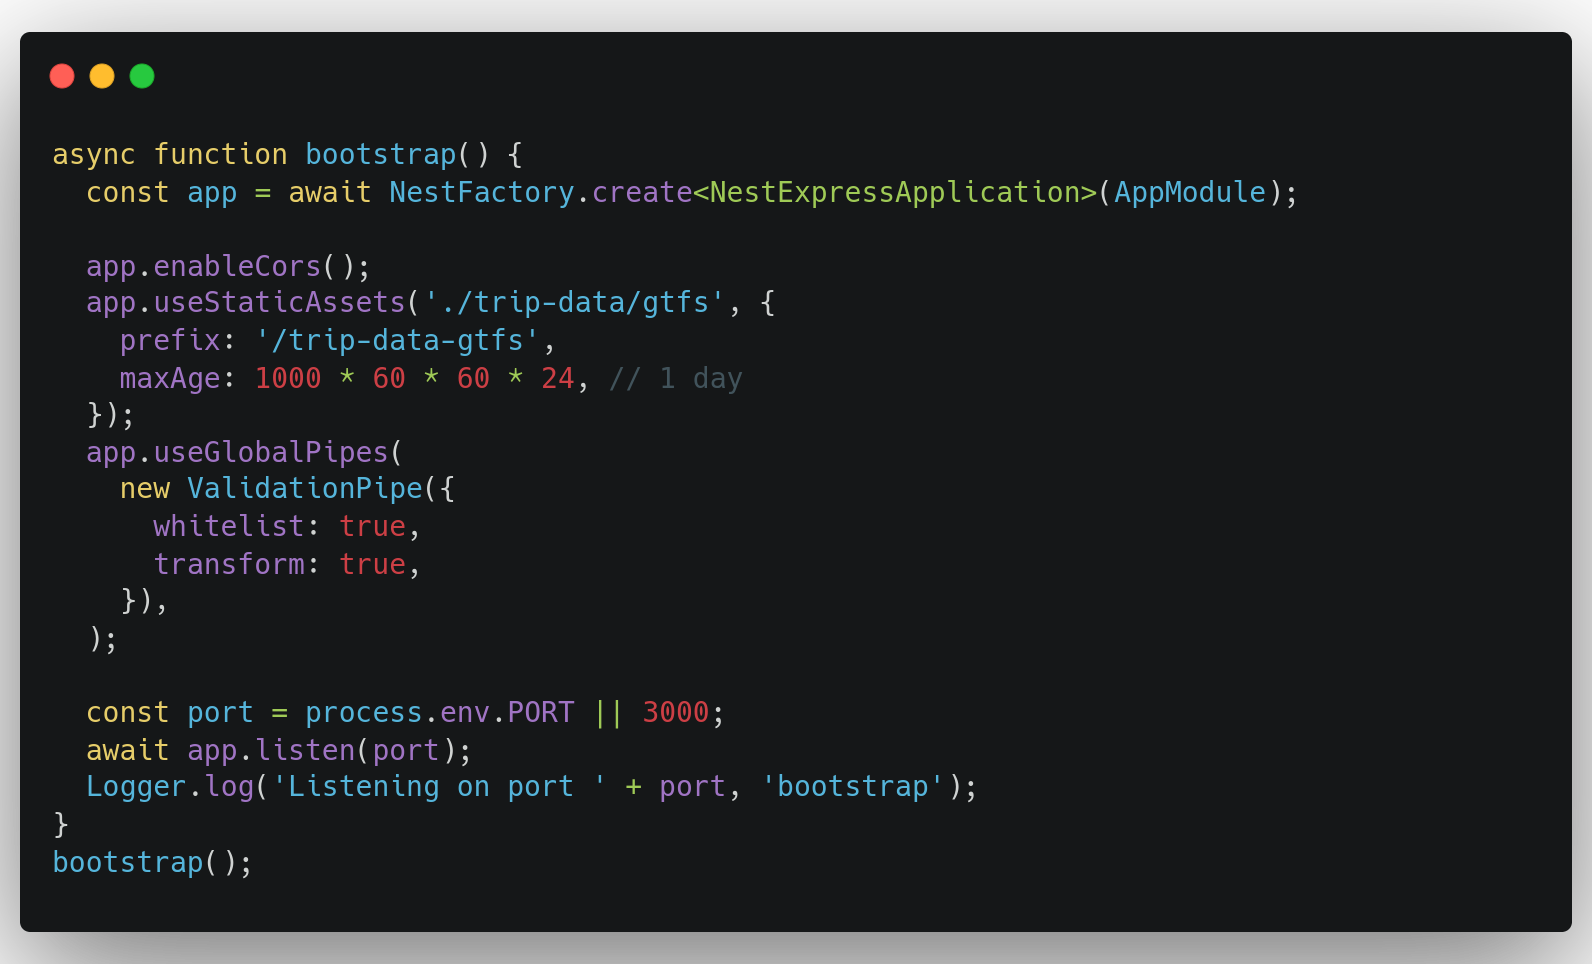
\includegraphics[width=0.9\textwidth]{./figures/code/be_bootstrap.png}
    \caption{Backend: bootstrapping code.}
    \label{FigBeBootstrap}
\end{figure}

Module definitions are not much more complex than importing all the dependency modules and adding them in the module definition, using the \verb|Module| decorator. The definition of the \verb|AppModule| is presented in Figure \ref{FigBeAppModule}, and consists of importing our three modules (auth, GTFS, and user) and the \verb|MongooseModule|, provided by Nest, which offers interaction with MongoDB databases, and the definition of the module class.

\begin{figure}[htbp]
    \centering
    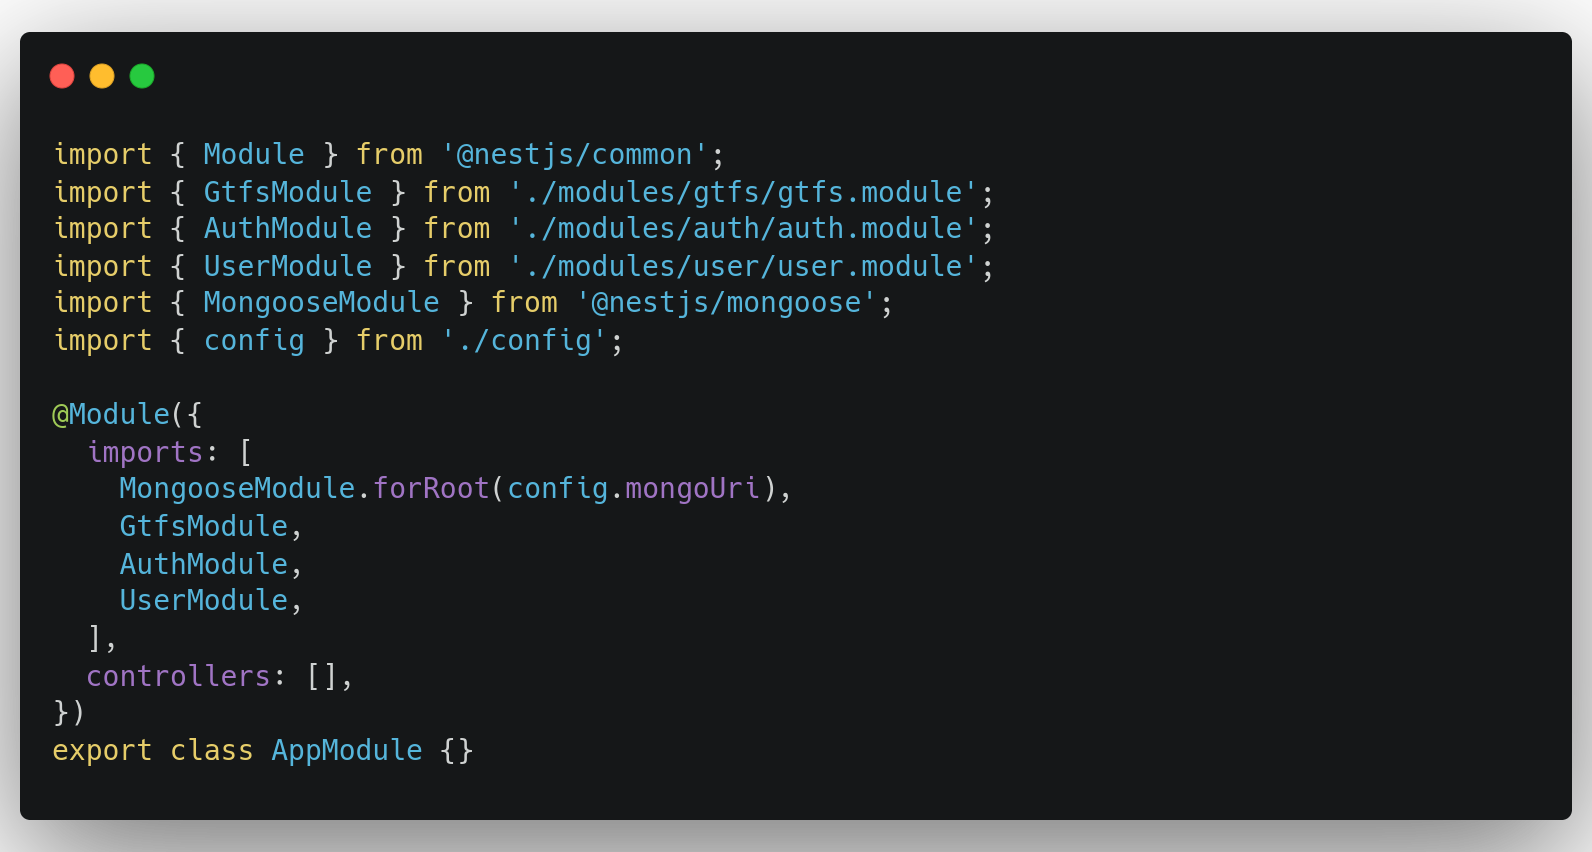
\includegraphics[width=0.9\textwidth]{./figures/code/be_app-module.png}
    \caption{Backend: AppModule.}
    \label{FigBeAppModule}
\end{figure}

\subsection{Configuration}
\label{sec:Configuration}

Backend configuration is stored in a \verb|config.yaml| file at the root of our project. The file is ignored by git, and serves as the location to place all the application secrets and connection instructions, along with configuration that might differ from an environment to the next.

A schema of the configuration file, without actual values, is presented in Figure \ref{FigBeConfig}. We can see configuration related to GTFS (where to download GTFS data from, and what files), along with social authentication secrets, MongoDB database URL, and JWT generation secret.

\begin{figure}[htbp]
    \centering
    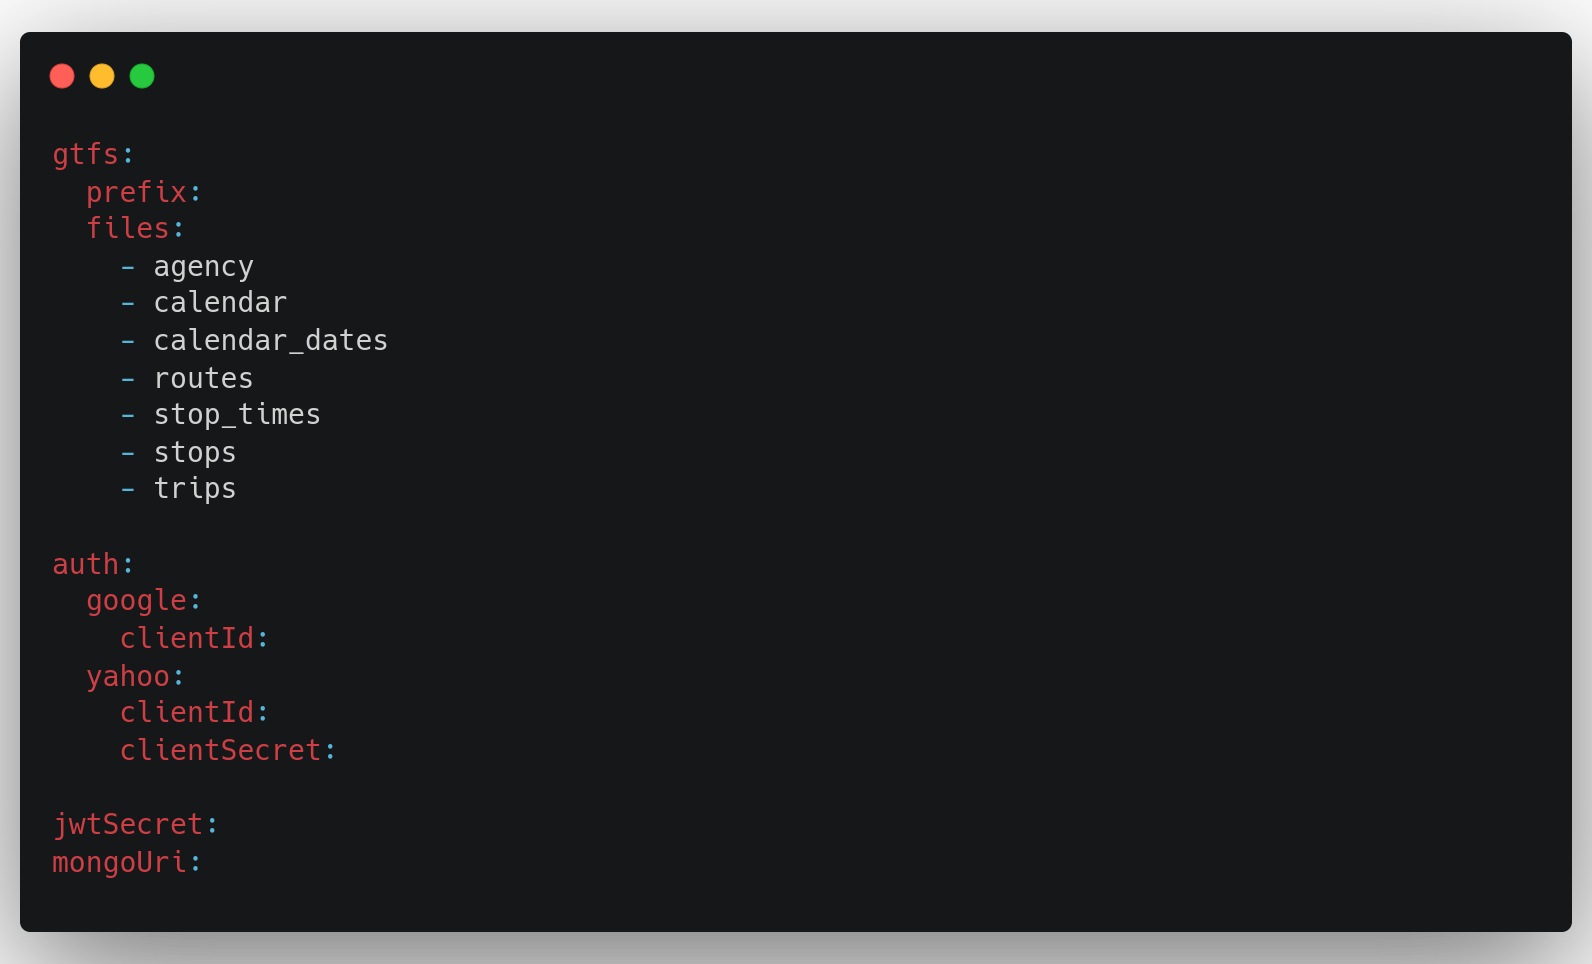
\includegraphics[width=0.9\textwidth]{./figures/code/be_config.png}
    \caption{Backend: config.yaml}
    \label{FigBeConfig}
\end{figure}

The YAML file is then loaded into memory in the \verb|config.ts| TS module, then exported so that it is available for the entire application.

Having the configuration file be loaded by Node is a decision taken in light of simplicity. NestJS offers ways of integrating configuration within its module system, but it requires writing additional code and logic, not only for the providing module, but for modules and services that use the configuration too.

As a safety precaution, the config file is validated against a schema using Joi, which can help identify missing configuration parameters at application startup, rather than have the application crash when it tries to access an inexistent configuration parameter. The Joi schema is presented in Figure \ref{FigBeConfigSchema}.

\begin{figure}[htbp]
    \centering
    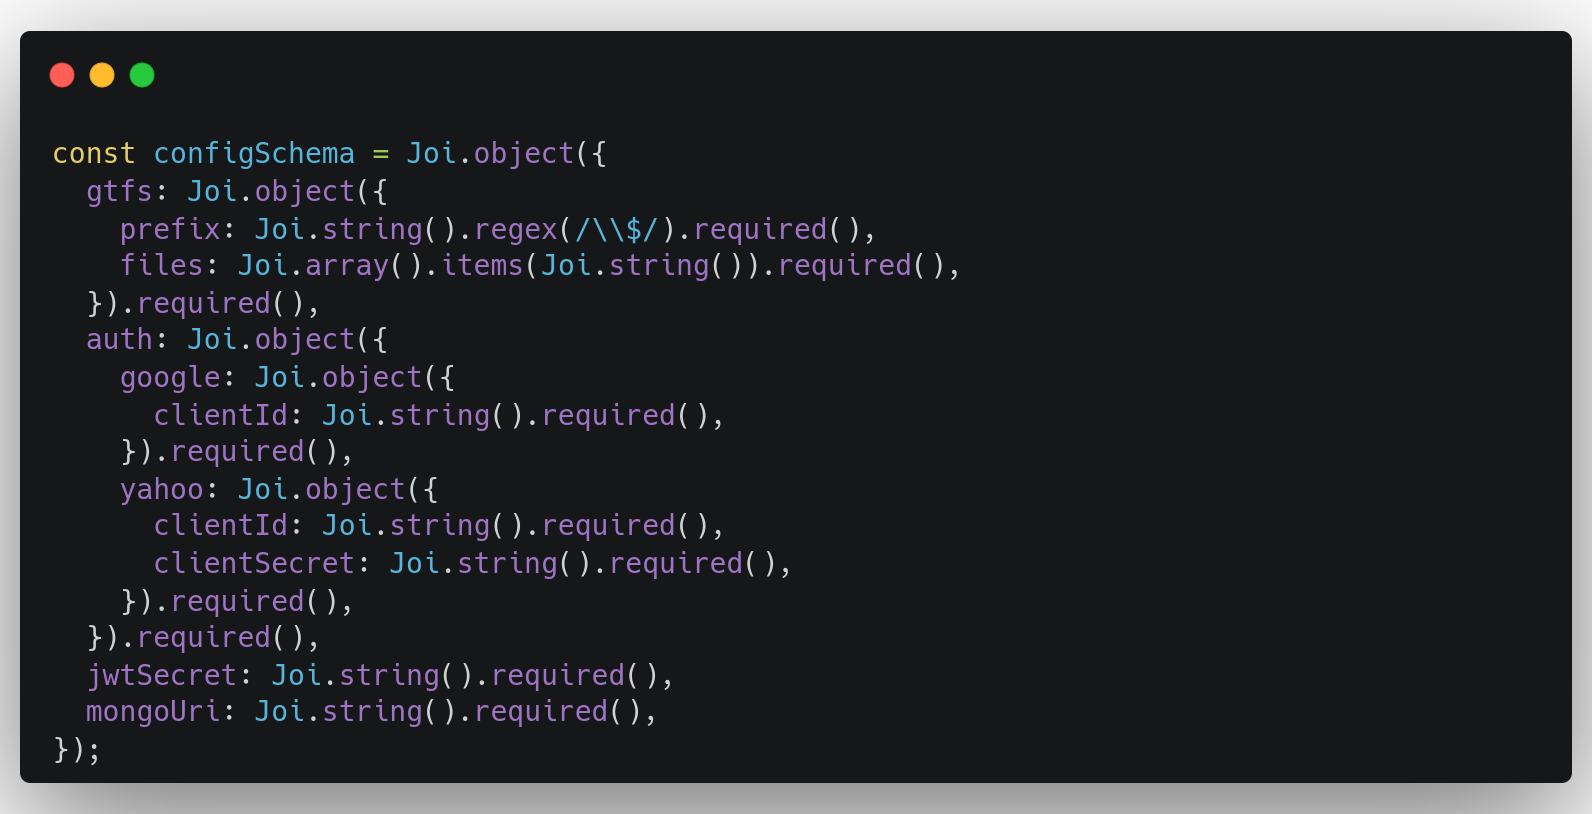
\includegraphics[width=1\textwidth]{./figures/code/be_config-schema.png}
    \caption{Backend: config validation schema.}
    \label{FigBeConfigSchema}
\end{figure}

\subsection{Preparing GTFS data for download}

The GTFS files are available on Vasile Coțovanu's GitHub repository \cite{VasileRubyExporter}, and before serving to our frontend, the files need to be downloaded locally first.

To this end, there exists a script called \verb|process-gtfs.ts|, that when run, creates a Nest application but only loads the GTFS module (Figure \ref{FigBeGTFSBootstrap}). The script then retrieves the \verb|GtfsService| service and uses it to initiate the download of GTFS data from GitHub, which is then placed in the \verb|trip-data| directory. This directory is then referenced in the static assets declaration from the application bootstrapping code (see Section \ref{sec:AppModule}).

\begin{figure}[htbp]
    \centering
    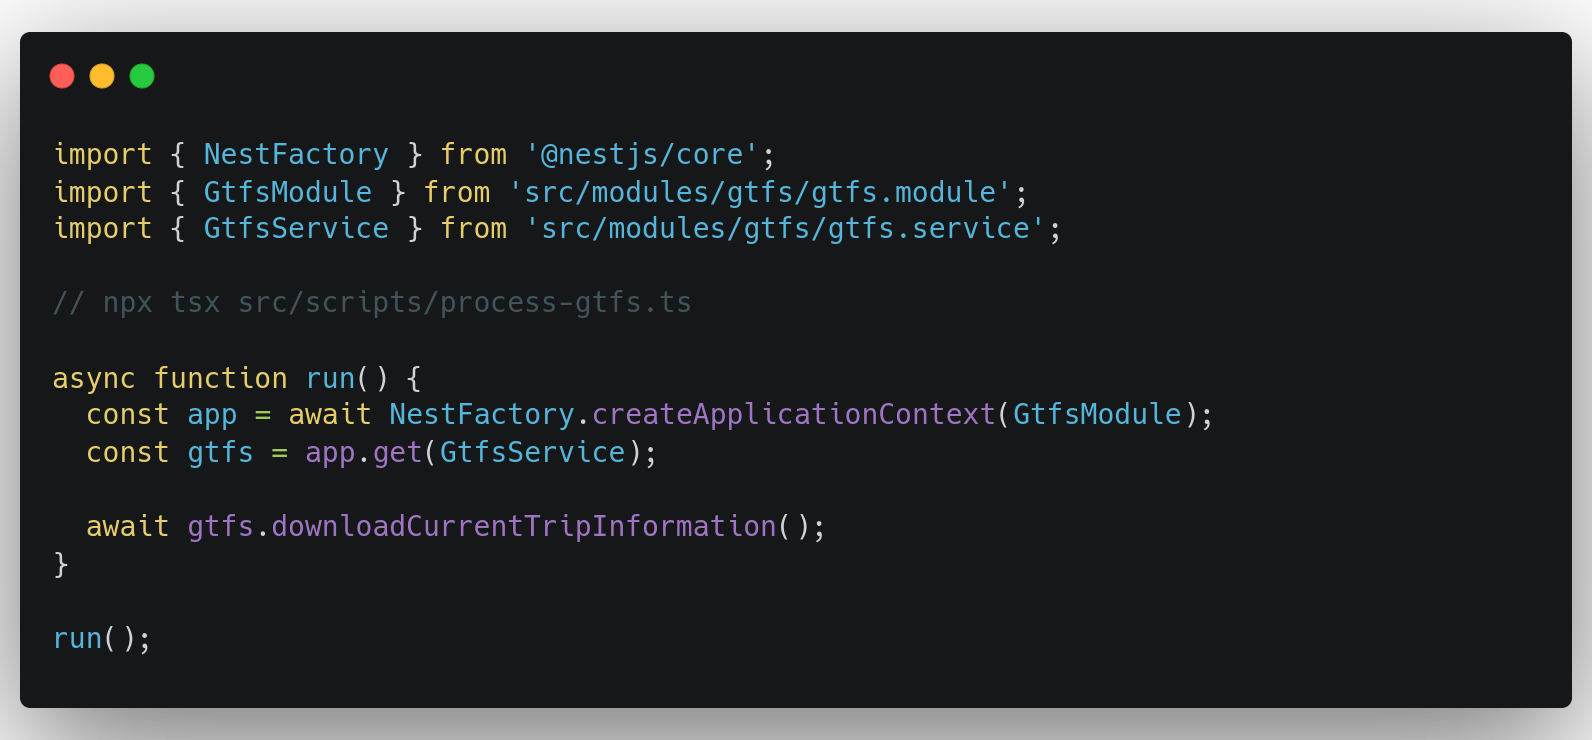
\includegraphics[width=1\textwidth]{./figures/code/be_gtfs-bootstrap.png}
    \caption{Backend: GTFS script bootstrapping code.}
    \label{FigBeGTFSBootstrap}
\end{figure}

\subsection{Auth module}

\begin{figure}[htbp]
    \centering
    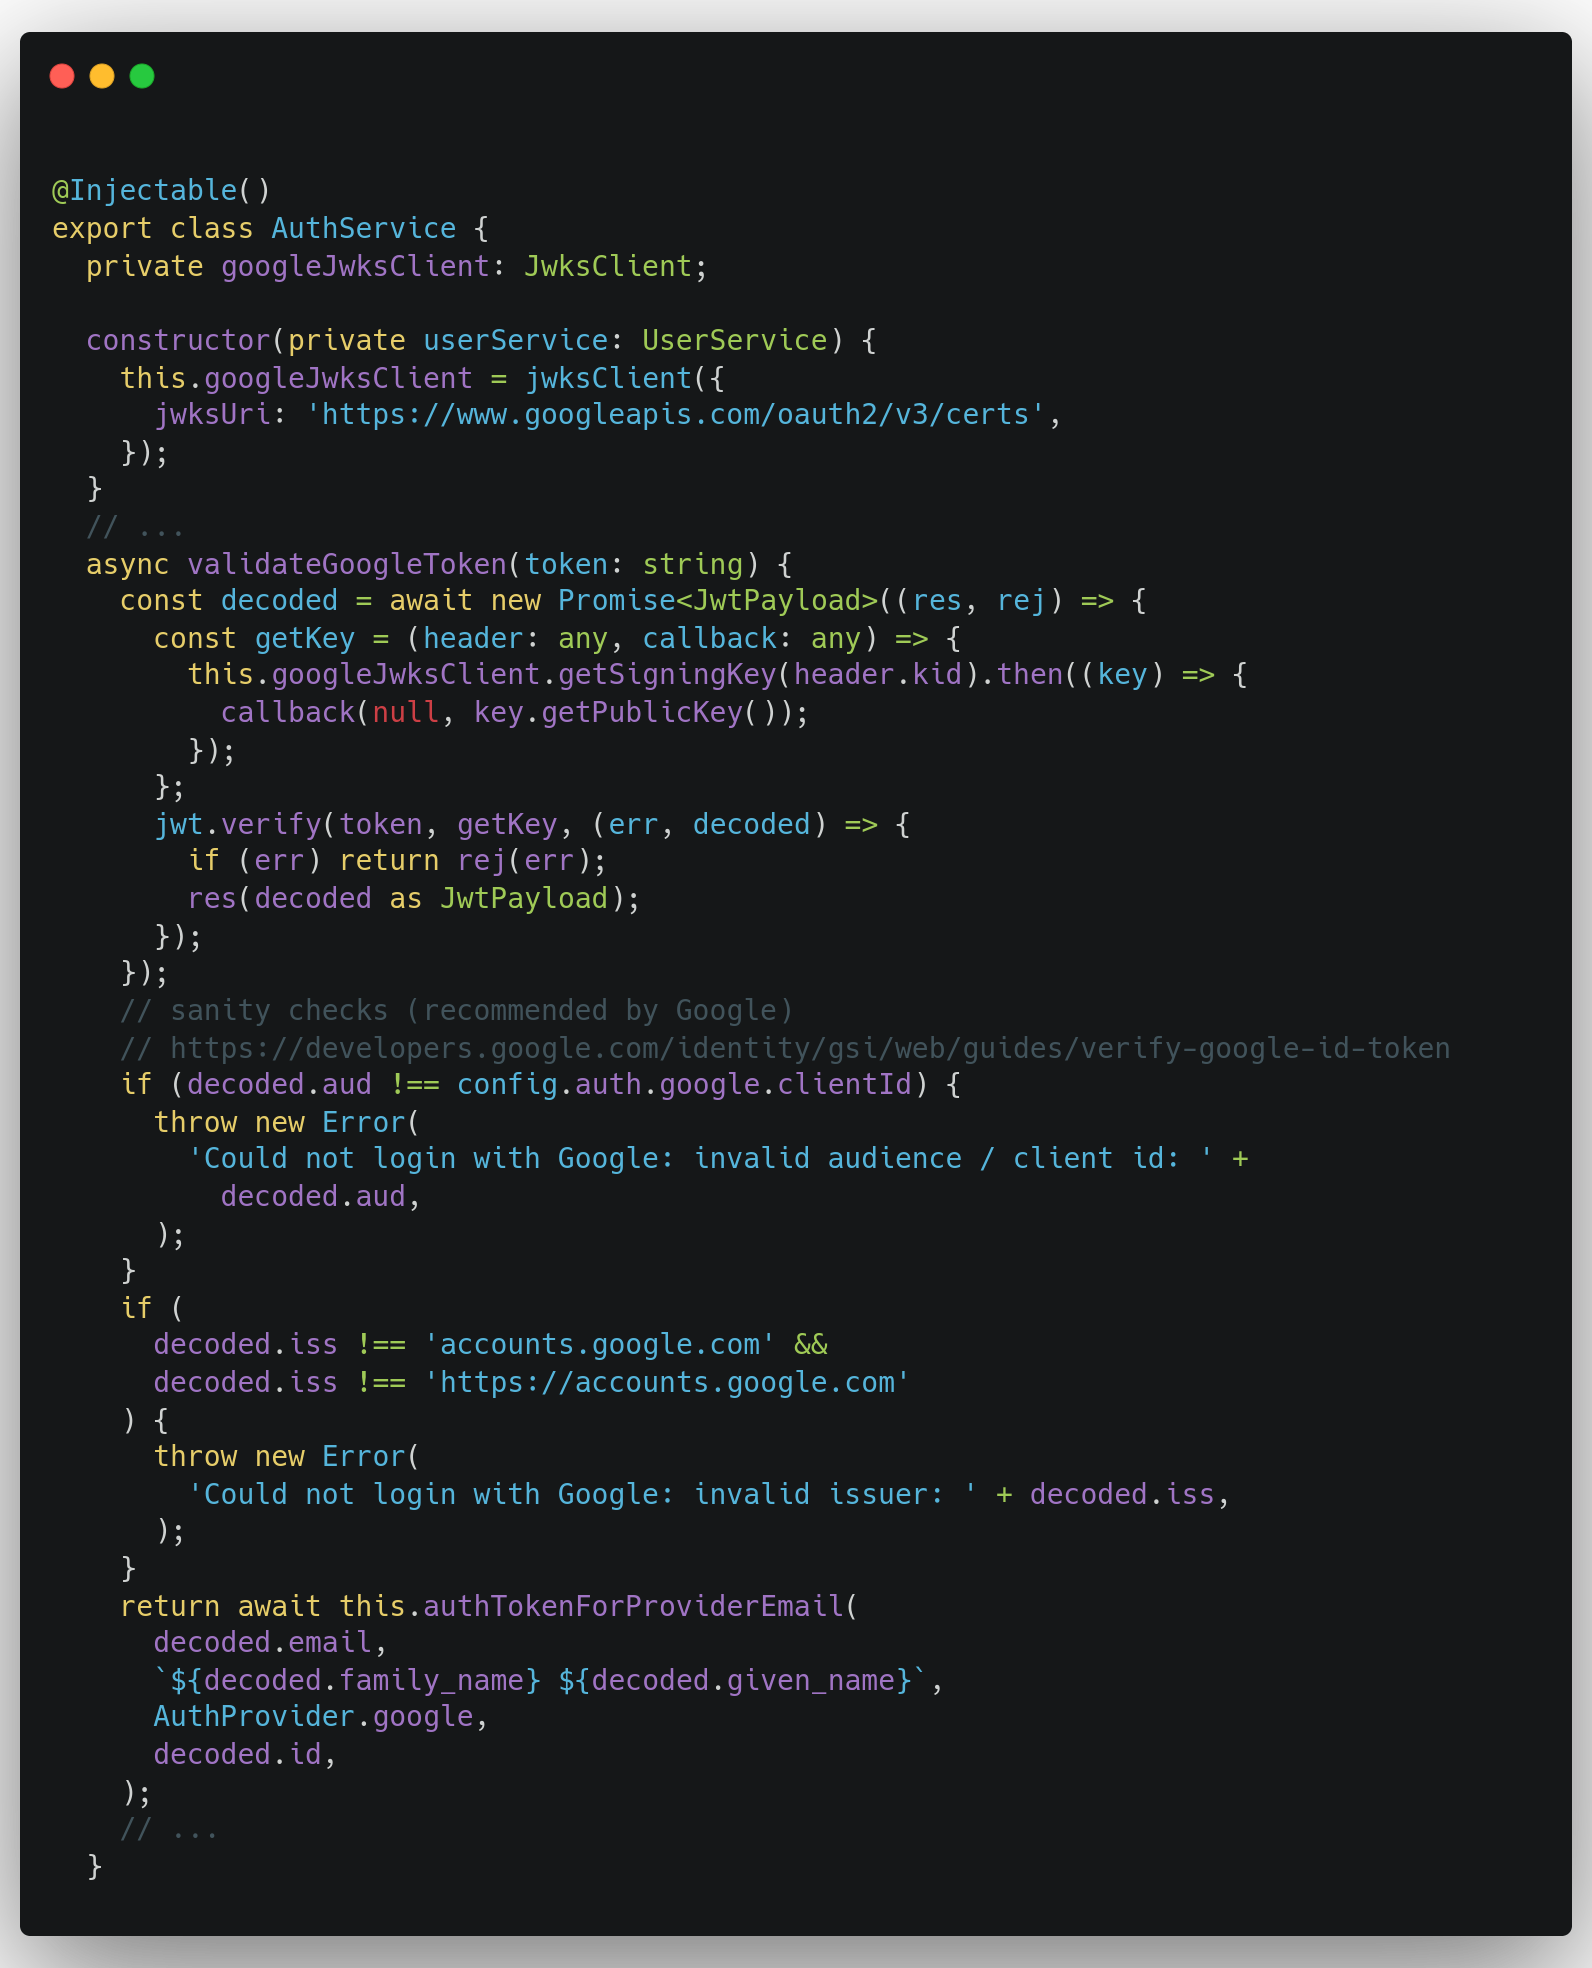
\includegraphics[width=0.9\textwidth]{./figures/code/be_auth-service-google.png}
    \caption{Backend: code that validates Google JWT tokens, for Google sign-in.}
    \label{FigBeAuthServiceGoogle}
\end{figure}

The Auth module has functionality related to user authentication: validating social logins, validating username and passwords, generating JSON Web Tokens (JWTs) and validating those tokens.

Google Sign-in is validated using a token received from the frontend and emitted by Google. The token is a JWT that is encoded using a JSON Web Key (JWK). Google publishes the public keys they use in a JSON Web Key Set (JWKS) format, which can be used to validate JWT tokens emitted from them, and verify their authenticity. Google also recommends performing a set of sanity checks on the JWTs apart from checking their signature, to prevent various attacks, such as emitting valid JWTs for a different application, or from a different Google service. The JWT signature verification library used in the app also makes sure that \verb|iat| and \verb|exp| are enforced (disallowing expired tokens). See Figure \ref{FigBeAuthServiceGoogle} for a code snippet of this step.

Yahoo Sign-in is validated by redirecting the user through a traditional OAuth authorization flow. At the end of the frontend flow, the backend receives a code that will then be sent to Yahoo (using a REST API) for validation, resulting in an \verb|access_token| that grants permission to Yahoo's OAuth APIs. The backend then makes a request to the userinfo endpoint, retrieving the user's email.

Upon validating social credentials, the backend then checks for an user account that already exists in the database (matching using the user's email as received from the social provider), creating one if one doesn't already exist. For this user id, a JWT token is emitted using the application secret (as defined in the configuration, see Section \ref{sec:Configuration}), and returned to the frontend.

The \verb|AuthModule| also provides methods to verify user JWTs, and a Request Guard that can be used to guard API routes that require authentication. Validating JWTs from API requests is done via a library called \verb|passport| and its Nest integration \verb|@nestjs/passport|. Making use of the JWT passport strategy, we can easily configure a strategy that checks JWTs received in the \verb|Authorization| header, via the application's JWT secret. The code is available in Figure \ref{FigBeJwtStrategy}, where it can be noticed how we configure \verb|passport| to validate JWTs, and tell it how to retrieve a user from a valid JWT by making use of the \verb|AuthService|.

\begin{figure}[htbp]
    \centering
    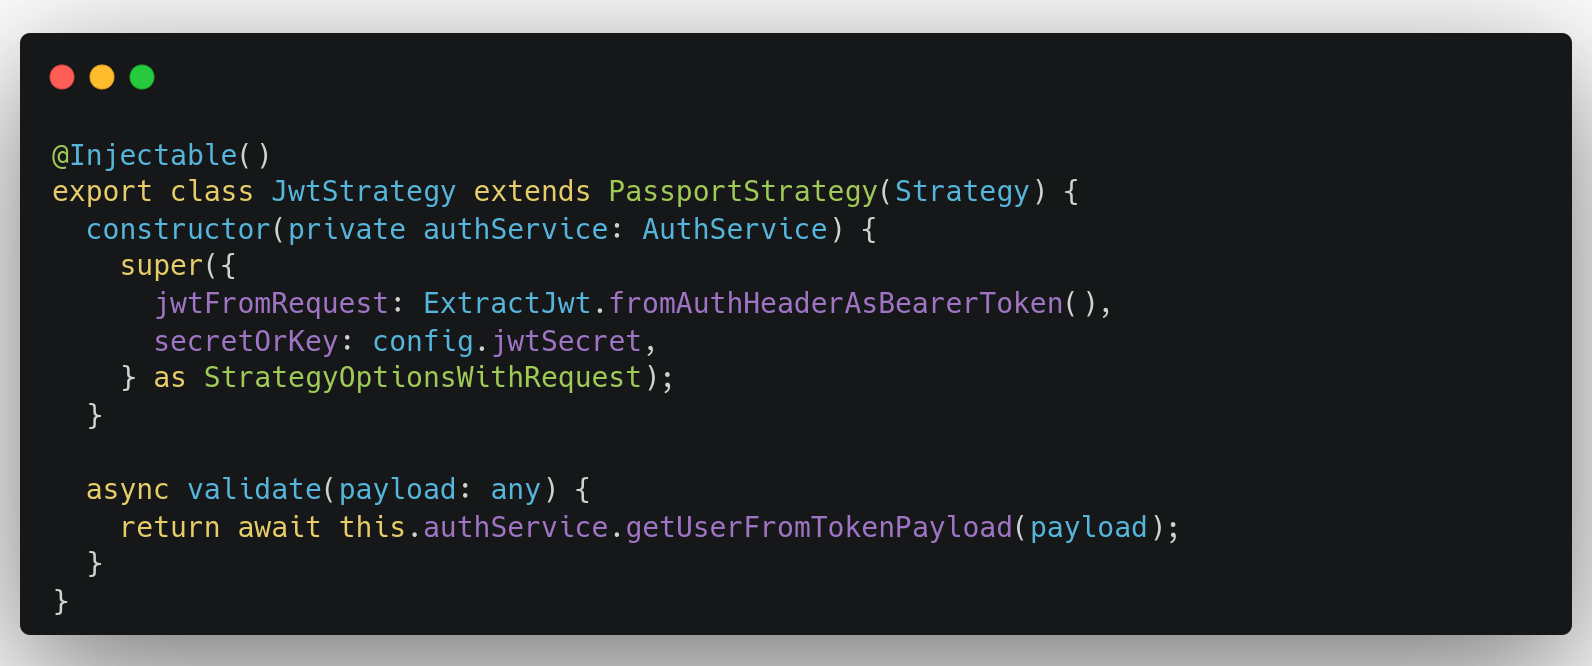
\includegraphics[width=1\textwidth]{./figures/code/be_jwt-strategy.png}
    \caption{Backend: the JWT strategy, as defined using @nestjs/passport.}
    \label{FigBeJwtStrategy}
\end{figure}

A popular method of accessing user data pertaining to a request, in the Express framework, is by attaching a \verb|user| property on the \verb|req| (Request) object. This object is passed around to all handler code in the app, making it an easy way of passing request state around the application. Nest abstracts away this \verb|req| object, and although it provides ways of accessing it, they are discouraged in lieu of a more opinionated approach, that is less prone to type errors. The Nest approach of decoding the user from the request consists of creating a decorator that makes this decoding for us, and places the user object into a parameter of choice in the controller code. The definition of this decorator, along with an example, is shown in Figure \ref{FigBeReqUser}.

\begin{figure}[htbp]
    \centering
    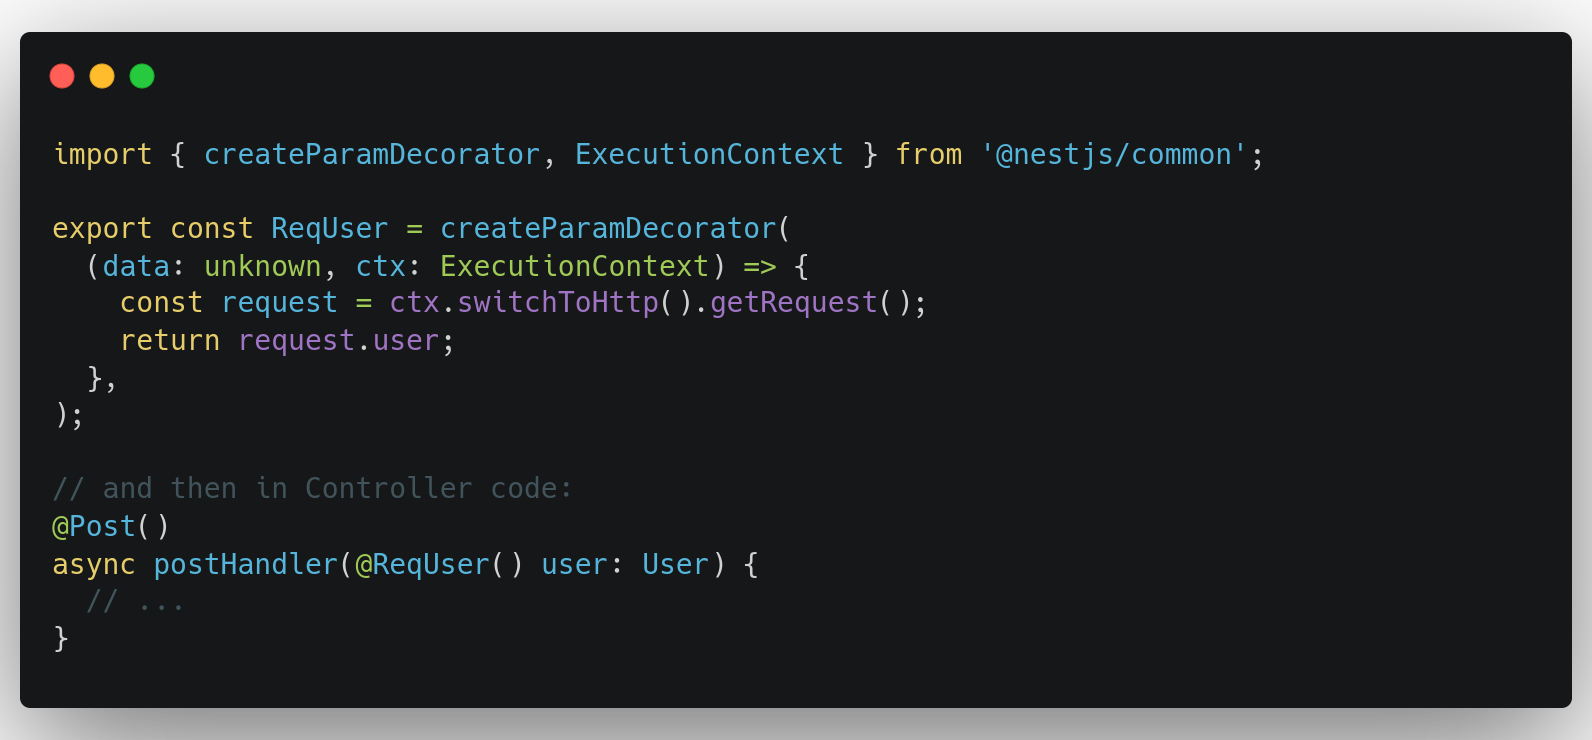
\includegraphics[width=1\textwidth]{./figures/code/be_req-user.png}
    \caption{Backend: the definition of the @ReqUser() decorator, along with an usage example.}
    \label{FigBeReqUser}
\end{figure}

\subsection{DTO validation}

All request validation throughout the app is performed using Data Transfer Objects (DTOs), that are decorated with specific validation criteria.

\begin{figure}[htbp]
    \centering
    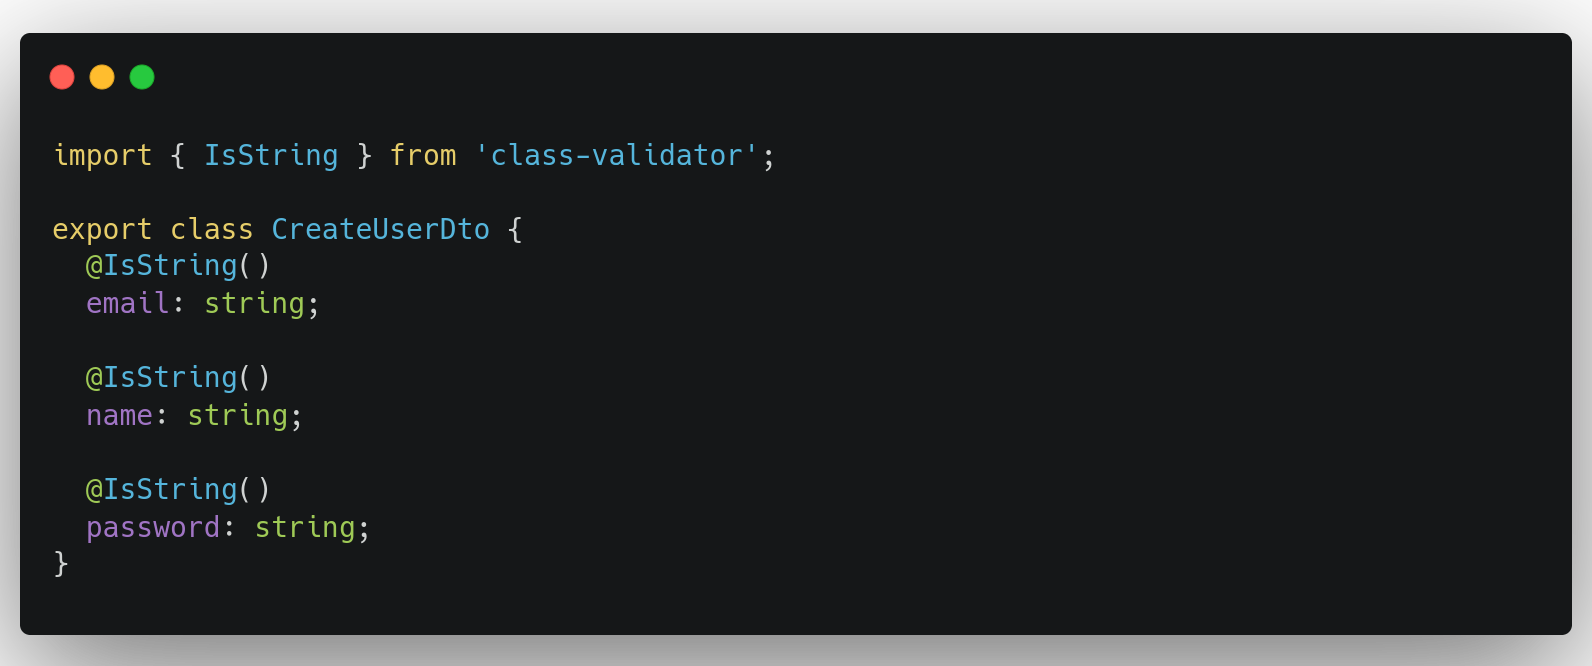
\includegraphics[width=1\textwidth]{./figures/code/be_dto.png}
    \caption{Backend: the definition of a DTO with validation, exemplified on the register request.}
    \label{FigBeDto}
\end{figure}

Figure \ref{FigBeDto} shows how such a validation class looks like. The \verb|ValidationPipe| declared globally (referenced in Section \ref{sec:AppModule}) will use this class decorated with \verb|class-validator| validators to validate the request body of the register endpoint. If a property is found to have a different type to the one specified in the constraint, \verb|class-validator| will throw an error and Nest will return a HTTP 422 status code, with detailed information about how the payload is malformed.

You can notice that the class fields are annotated with TypeScript types (in this case, string). It is important to point out that these types are not enforced at runtime, since they only aid in compile-time type safety. There is nothing to prevent the programmer from adding TS types here that do not match with the decorators, however this mistake is unlikely due to how the decorators are placed right next to the properties.

A special kind of attack can be performed by adding more properties on the request body object that have special significance to other components of the application (for example, MongoDB). By default, the ValidationPipe provided by Nest only checks that those three fields (email, name, password) are valid, but once these checks are complete, the entire request body is deserialized and converted into a JS object, with all its properties. It's then trivial for those properties to be passed to \verb|mongoose| database code, as a byproduct of language features such as the spread syntax (\verb|...obj|), and then have them run arbitrary queries on the database system. To this end, the ValidationPipe offers a configuration parameter \verb|whitelist|, that will remove all extraneous properties that are not explicitly validated in the DTO. If unvalidated properties are desired, the programmer can use the \verb|@Allow()| decorator.

\subsection{User module}
The user module handles users and their trips. The trips are not separated in another module due to how they are stored in the database under the same document, and thus are accessed using the same MongoDB collection (or model, as described by \verb|mongoose|).

\begin{figure}[htbp]
    \centering
    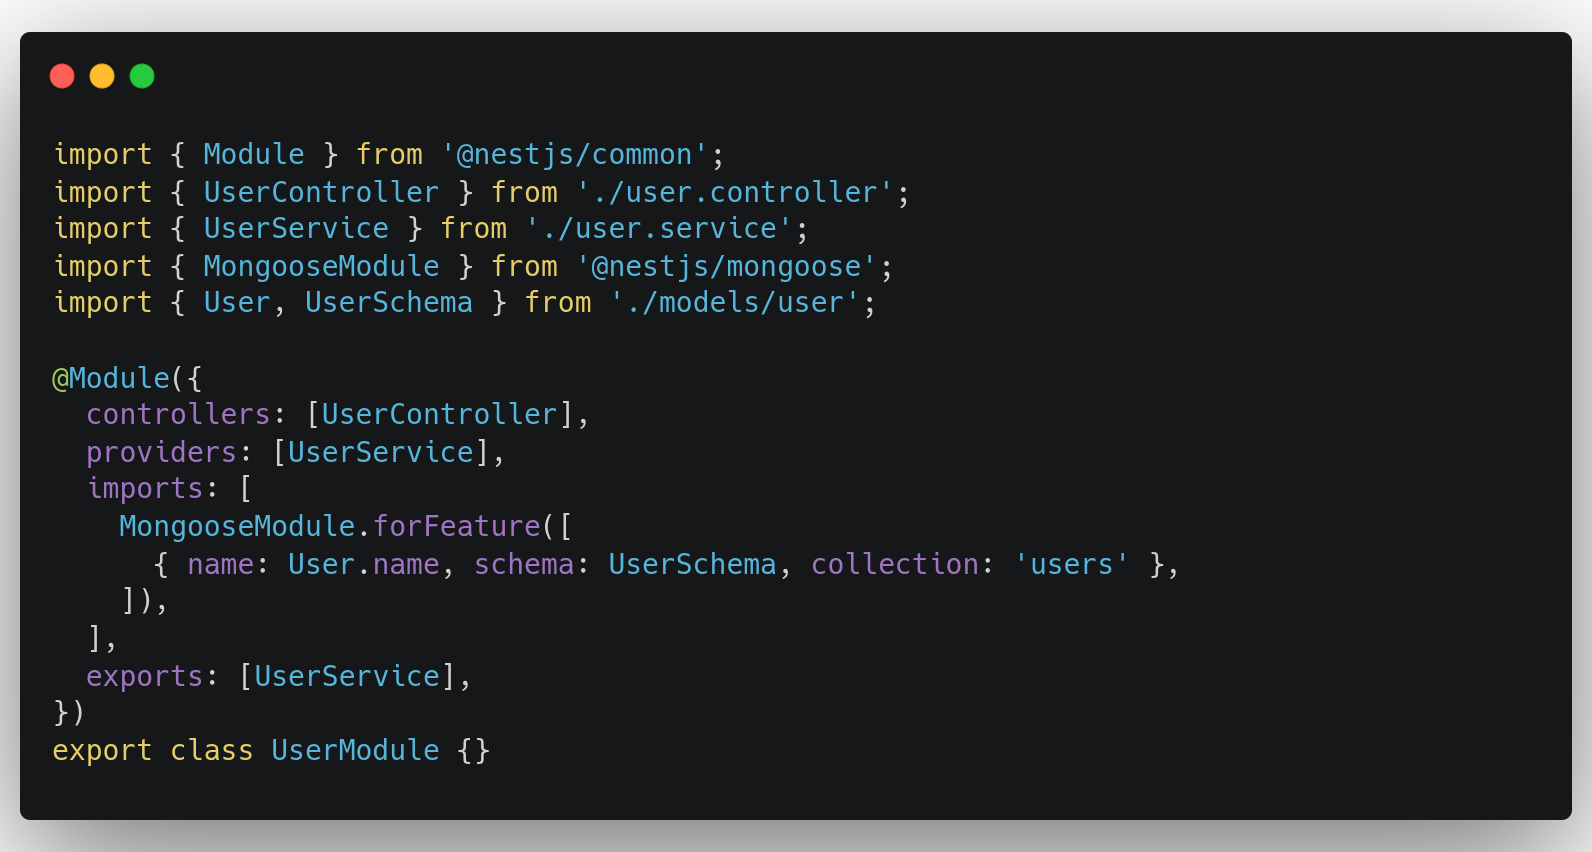
\includegraphics[width=1\textwidth]{./figures/code/be_user-module.png}
    \caption{Backend: the user module.}
    \label{FigBeUserModule}
\end{figure}

Figure \ref{FigBeUserModule} shows the definition of the UserModule. It is interesting to notice the separate parts of the module declaration:
\begin{enumerate}
    \item \textbf{controllers:} represents the list of controllers that this module exposes to the Nest framework. Controllers that are not registered here are not visible to Nest's internal router.
    \item \textbf{providers:} represents the list of providers that this module makes use of. A provider is any class decorated with \verb|@Injectable()|, and all providers are available for dependency injection.
    \item \textbf{imports:} represents a list of modules that this module depends on. Namely, we depend on MongooseModule. However, registering MongooseModule as a root module is not suitable here, since we already imported it as root in AppModule. For this reason, we use \verb|.forFeature()|, which is used to register specific models for use with \verb|mongoose|.
    \item \textbf{exports:} represents a list of all providers that this module exposes to other modules. As a consequence, all modules that import UserModule have access to the UserService. The module that makes use of this service is the AuthModule.
\end{enumerate}

Another interesting analysis we can make is on the User model. The \verb|mongoose| framework makes use of \textit{schemas} to enforce object validation on the documents that get persisted to the database. However, the schemas need to be declared in plain JavaScript, and since they don't integrate well with TypeScript, the mongoose documentation recommends writing the schema twice: once for registering in mongoose, and once for TypeScript type safety.

Nest offers native support for mongoose, and comes with a solution to enable a single class to provide both a mongoose schema, and TypeScript type safety. Visible in Figure \ref{FigBeUserModel}, the solution consists of decorating all class properties using the \verb|@Prop()| decorator, in a manner not unlike the validation performed by the validation library \verb|class-validator|.

All the \verb|@Prop()| arguments are directly passed to mongoose, so as to make the abstraction as minimal as possible. Similarly, all arguments to \verb|@Schema()| are passed to the mongoose Schema constructor.

In this manner, the class is already ready for TypeScript, and only awaits conversion to a mongoose Schema with the Nest \verb|SchemaFactory.createForClass()| method, seen in action in the last line of Figure \ref{FigBeUserModel}.

\begin{figure}[htbp]
    \centering
    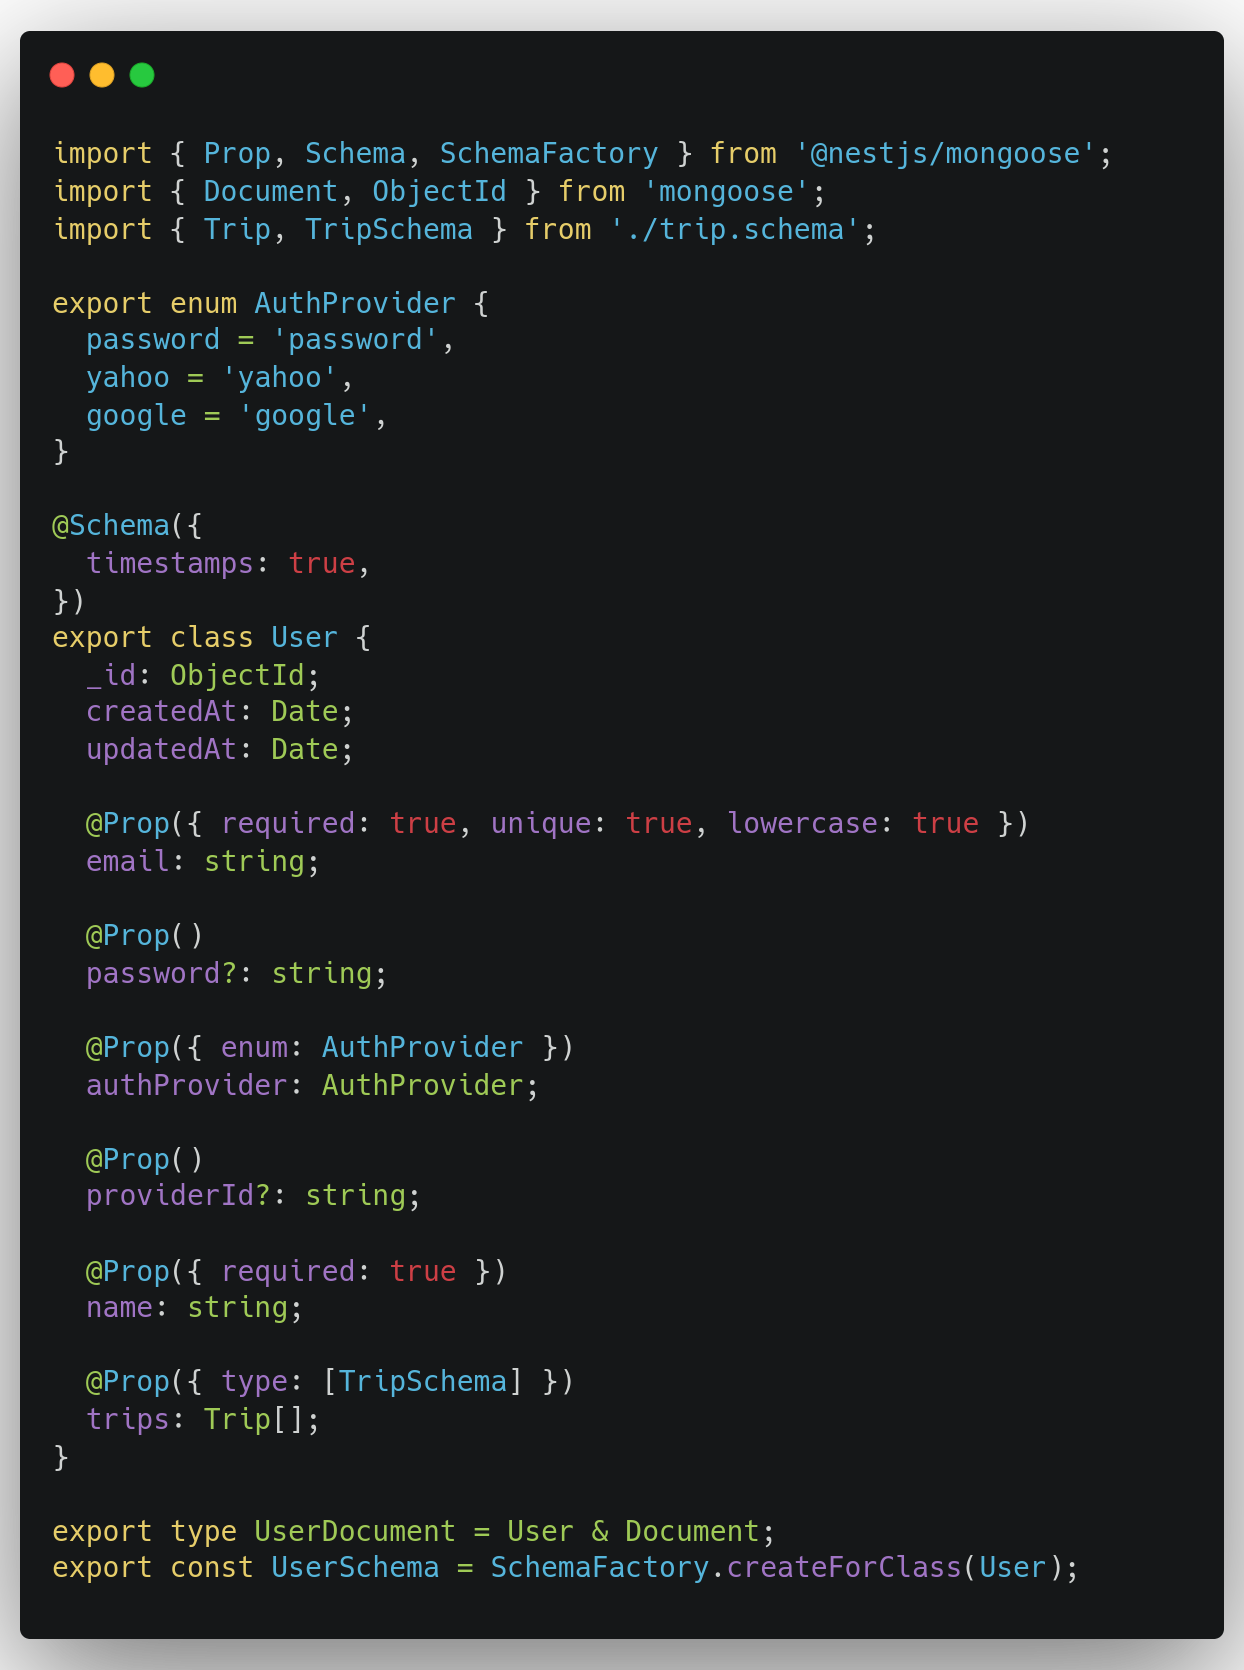
\includegraphics[width=.8\textwidth]{./figures/code/be_user-model.png}
    \caption{Backend: the user model.}
    \label{FigBeUserModel}
\end{figure}

\subsection{Building the project}

Since we employed TypeScript in the project, we are now required to compile the project in order to make it runnable. Albeit running the project directly (the TS files) is possible using tools such as \verb|ts-node| or \verb|tsx|, these tools compile the code on-the-fly, thus making the overall execution slower.

This being said, the compilation does not involve any additional steps apart from the TypeScript compilation.

As such, compiling the project is as easy as running \verb|npm run build| from the root directory of the project. This compiles all TS code and outputs it in the \verb|dist| directory. One can now run \verb|dist/index.js| directly, or use \verb|npm start|, to start the server.

\subsection{Deployment of the backend}
\label{sec:BeDeployment}
Deployment of the backend infrastructure is an interesting case study.

For one, a happy consequence of having the database deployed in the cloud separately is how we don't need to create any special infrastructure for it, since just passing the correct connection URL to the backend application is sufficient for it to successfully connect to it. The database connection is sufficiently fast, even across the Internet (as opposed to on the local computer or even network), as long as the backend and frontend are roughly in the same geographic region (eg. Frankfurt, where both DigitalOcean and Atlas have data centers).

For another, there are cost restrictions imposed on the deployment. I personally own a DigitalOcean droplet (virtual machine in the cloud) that I use for all my projects, so as to have a fixed monthly costs regardless of traffic.

As such, the steps I use to deploy the backend is as follows:
\begin{enumerate}
    \item If first time, clone the repository on the remote machine. Otherwise, just git pull.
    \item Run \verb|npm i| to download or update dependencies.
    \item If first time, make sure the \verb|config.yaml| configuration is suited for production.
    \item Build the project.
    \item If first time, create a \verb|ecosystem.config.js| file, telling PM2 how to run my app (see Figure \ref{FigBeEcosystemConfig}). PM2 is the process manager I use on the VM, that handles app restarts, logs and monitoring.
    \item Run the project using PM2, letting it take over.
\end{enumerate}

\begin{figure}[htbp]
    \centering
    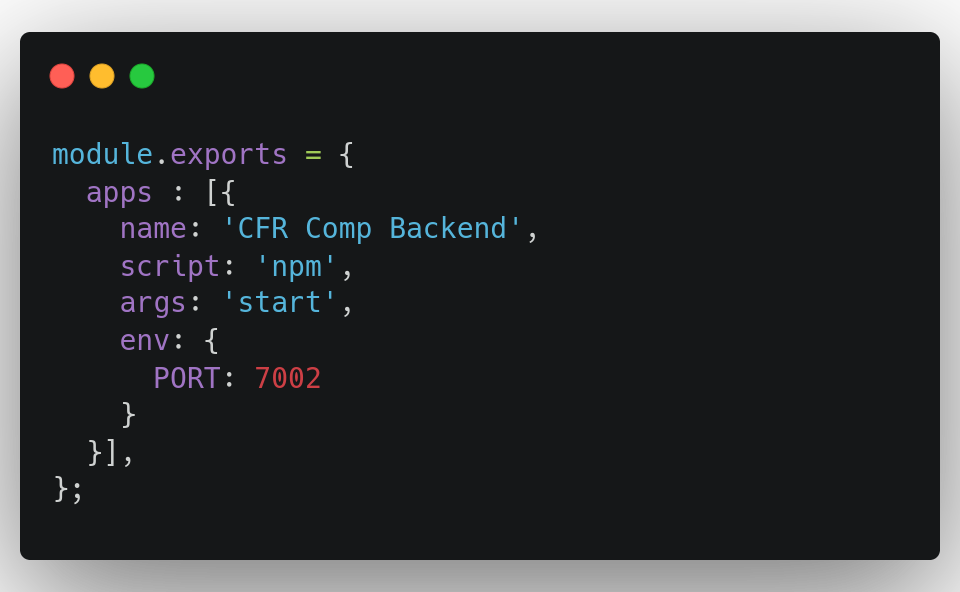
\includegraphics[width=.8\textwidth]{./figures/code/be_ecosystem-config.png}
    \caption{Backend: the ecosystem config, used by PM2 on my personal VM instance.}
    \label{FigBeEcosystemConfig}
\end{figure}

Having a shared virtual machine as a deployment environment proves a challenging task for any continuous integration / continuous development pipelines setup. For this task, I used an application specifically to handle this odd deployment scenario, called Deploy Monkey, available on GitHub \cite{DeployMonkey}. This custom application can link GitHub Actions (by use of webhooks) with my droplet, such that my droplet can automatically run the steps defined above locally, upon notification from GitHub that a push happened.

\section{Frontend application}
Arguably being the most important part of the application, the frontend is written in React with TypeScript and is written to be conformant to the PWA specification, so that it possesses the qualities of a PWA: installable and functional offline.

The bundler used is Vite. The role of a bundler is to take all the different source files and "bundle" them together in a single monolithic file, while also passing the code through all the required compilation steps. In this case, Vite also offers features to help with the development experience, such as hot reloading, and a local web server.

For our purposes, Vite also offers a plugin that helps us convert our application into a Progressive Web Application. We'll explore how this has been done in its own subsection.

\subsection{Functional code}
Modern React does not make use of classes as much as previous versions of it did. In the newer iterations of the library, components are not represented by JS classes anymore, but rather functions, which take the intuitive name of functional components.

\begin{equation}
    \label{eq:StateView}
    f(state) = view
\end{equation}

While classes were the de-facto standard way of writing React code for a long time, they lead to a lot of boilerplate code that could easily have been avoided using functional components. These components were possible back then too, but they were extremely limited in functionality and capability, until React unveiled \textit{hooks}, which changed the functional component scene.

Functional components are extremely intuitive due to how they closely map to the identity presented in Equation \ref{eq:StateView}. In the same manner that a view is a function of the state, a React functional component is a function that returns JSX code based on its parameters (or, how React calls them, \textit{props}).

While, in an ideal world, the above identity would be sufficient to write applications, it must be recognized that React components must do extra things other than calculate views based on their props. As such, React exposes a variety of hooks, that can be called from functional components. These hooks are normal JavaScript functions that "hook" into the React framework and let your functional component keep its own state, make it react to changes in props (or state), or let it perform side-effects as a result of state changes (eg. API calls).

These hooks, while normal JS functions as far as the language is concerned, do carry additional responsibility, due to the way they work with the framework. These restrictions are synthesized into the Rules of Hooks, and they look as follows:

\begin{enumerate}
    \item \textbf{All hook names must begin with 'use'.} For example, \verb|useState|, \verb|useEffect|.
    \item \textbf{Hooks must always be called in the same order.} React keeps track internally of this order to be able to return the correct values for consecutive render calls.
    \item \textbf{Hooks must never be called conditionally.} React will exhibit undefined behavior when a function render performs different hook calls than its previous render. There are situations where conditional hooks are desired, but they must be implemented differently, to avoid breaking the Rules of Hooks.
\end{enumerate}

Our application exclusively makes use of functional components, using hooks. Several custom hooks are also defined, that enable specific application functionality such as authentication, localization, or trip data updates.

\subsection{Pages}
Pages are laid out in a folder structure that closely reflects their URL, under the \verb|pages| directory. The website root layout is defined in the \verb|App.tsx| module, and it takes care of rendering the top navigation bar, along with rendering the child page using React Router.

Rendering of different pages was accomplished using React Router. Using this library is as easy as defining the hierarchy of pages, and using a couple of custom anchor link components instead of the HTML native \verb|<a>| tag.

Figure \ref{FigFeRouter} presents the routing definition, and it is easy to see how the App component is defined as the root page, with the children being the HomePage and TrackPage components.

An odd presence here is the YahooAuthPage, but it is justified by how the Yahoo OAuth authorization flow requires a callback URL to redirect to after the user grants permissions. This page will take the authorization code from the URL and pass it to the API.

\begin{figure}[htbp]
    \centering
    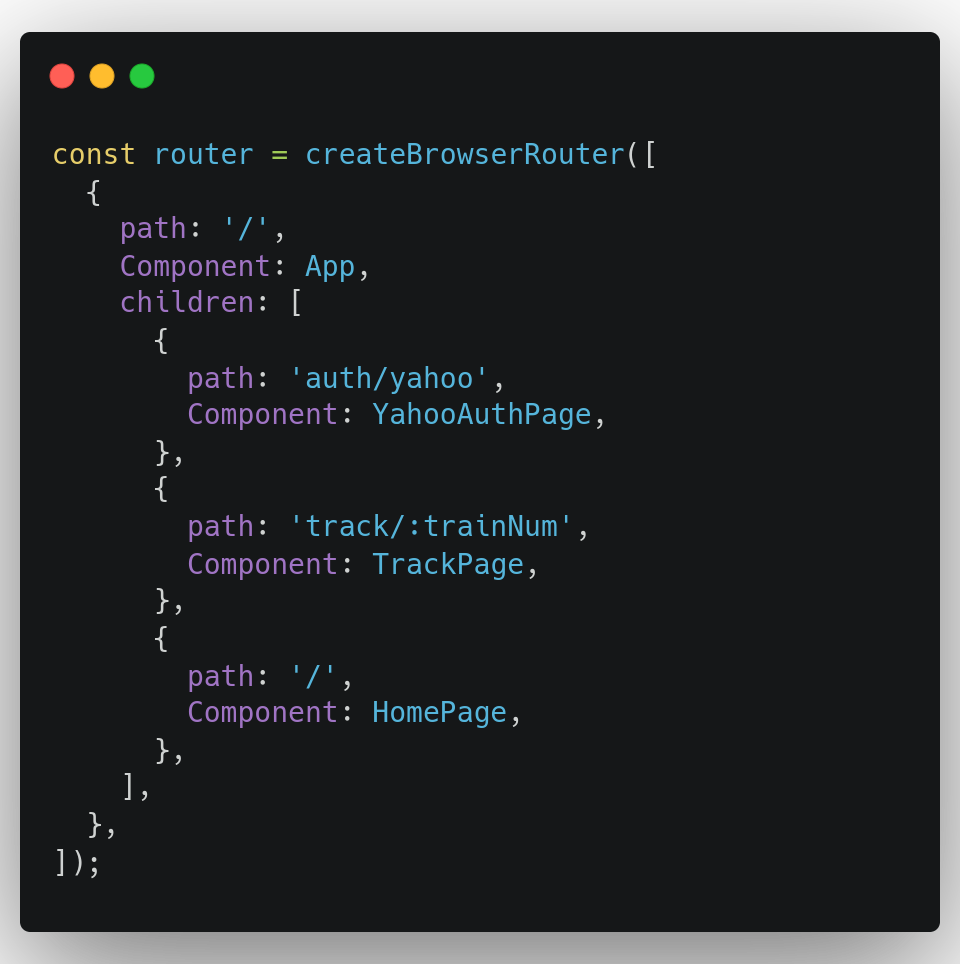
\includegraphics[width=.6\textwidth]{./figures/code/fe_router.png}
    \caption{Frontend: the application router.}
    \label{FigFeRouter}
\end{figure}

\subsection{Contexts}
While state can be declared in parent components and passed down to every component that needs it, state that is required in a lot of components across the component tree might require to be passed through components that make no use of it, and will generally lead to a phenomenon called \textit{prop drilling}.

While there exist a number of libraries that offer global state, such as \verb|zustand|, React does offer its own solution to this issue, in the form of \textit{contexts}.

A context takes the form of a plain JS object that can be declared at the top of the component hierarchy using a Provider, and that can be later accessed at any point in the tree using the \verb|useContext| hook.

Figure \ref{FigFeContexts} shows the React \verb|createRoot| call, and features all the context provi\-ders that the application makes use of. These provider components are plain functional components that keep their own relevant state, and that wrap their children in the React Context Provider component, which makes their state globally available.

\begin{figure}[htbp]
    \centering
    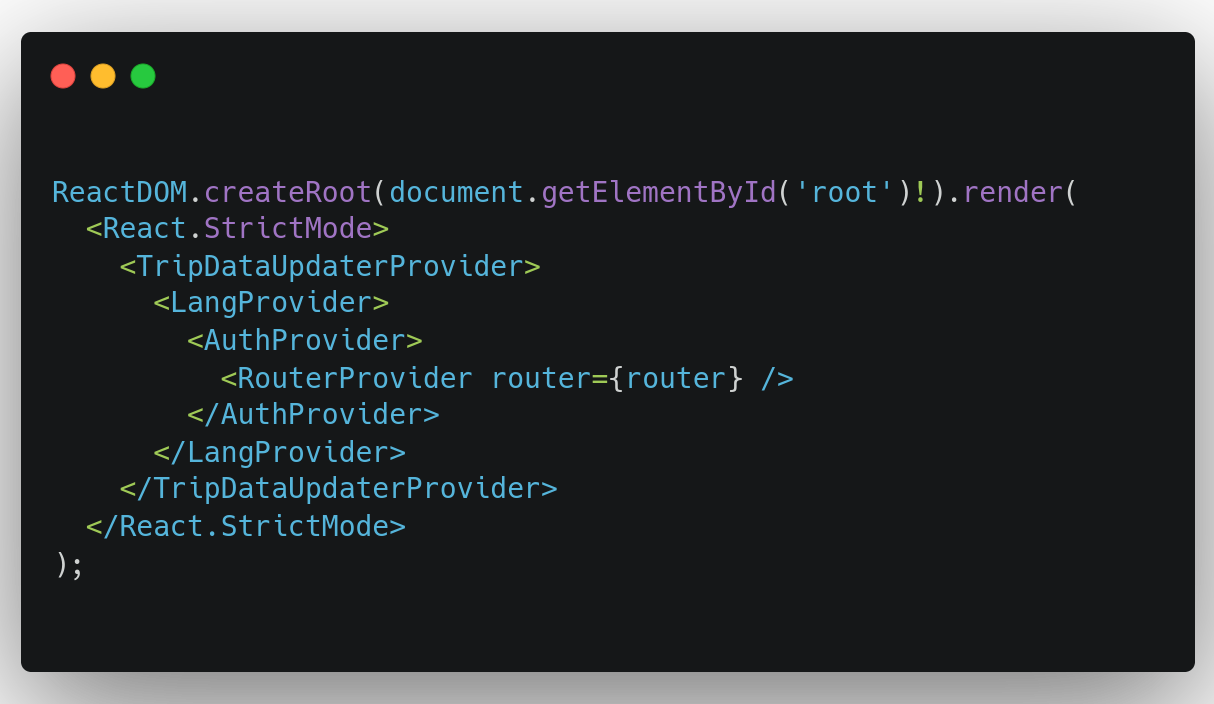
\includegraphics[width=.8\textwidth]{./figures/code/fe_contexts.png}
    \caption{Frontend: the createRoot call, featuring all the context providers.}
    \label{FigFeContexts}
\end{figure}

\subsection{IndexedDB wrapper: Dexie}
IndexedDB is a browser native capability, but its API is deemed to be somewhat hard to use. It technically is async, but has a lot of weird restrictions in place that prevent it to be used in a truly async fashion.

As a consequence, I have decided to use Dexie.js as a wrapper around the IndexedDB functionality. Dexie is able to handle different use cases, such as database migrations, minimal schema validation, TypeScript integration, and indexes. One bonus feature that helped during development was its integration with React, being able to hook into React state and run queries reactively.

\begin{figure}[htbp]
    \centering
    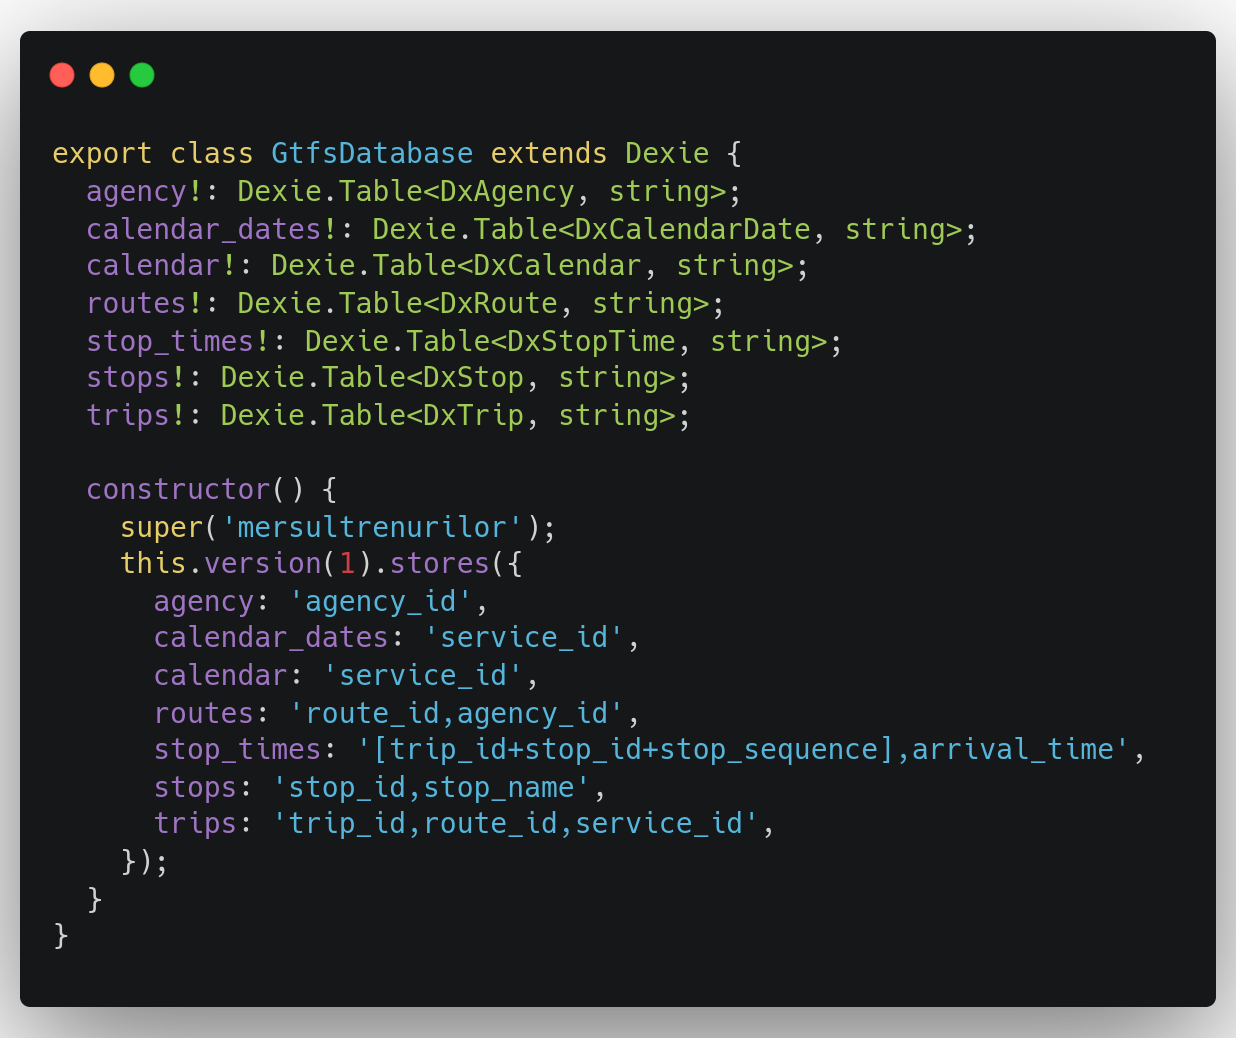
\includegraphics[width=.8\textwidth]{./figures/code/fe_dexie-gtfs.png}
    \caption{Frontend: setting up the Dexie GTFS database.}
    \label{FigFeDexieGTFS}
\end{figure}

Figure \ref{FigFeDexieGTFS} shows the declaration of the GTFS database class. It directly extends the Dexie class, meaning that it exposes all Dexie functionality, but in addition, on instantiation, it automatically sets up the database for use with our GTFS data.

The first few lines represent purely TypeScript support. To make TS aware of our tables, we need to explicitly tell it that they exist, and we provide a interface that it can then do type-checking against. The interfaces are all prefixed with \verb|Dx| to differentiate them from API entities.

The constructor then calls the parent constructor with the name of the database (\verb|mersultrenurilor|), which is followed by the schema definition. While Indexed\-DB does not make use of structured tables and schemas in the same manner as MySQL would, it does need to create tables and set up search indexes on them. Dexie will create all the tables listed in the \verb|stores| call, and set up all the comma-separated indexes. The first value of every enumeration will be considered a \textit{key}, which is functionally equivalent to a primary key in relational databases.

You can notice a special syntax in the \verb|stop_times| definition. That syntax has the effect of creating a \textit{composite primary key}, since all stop times are determined by their trip, stop, and stop sequence.

It is important to notice how the index lists are not covering the entire object they store. IndexedDB can store \textit{any} plain JS object, and it does not place restrictions on what shape those objects can have. As such, the indexes only take the role of a speed enhancement, and not of a restriction.

\subsection{Loading offline GTFS data}
Downloading the GTFS data is always done on page load. The application does a check online to see when the GTFS data has been last updated, and compares it to the last download date it has locally (in the IDB store). If there is newer data on the server, it downloads into memory the entire contents of the GTFS data files, and then uploads them into the IndexedDB database.

This process can take a while, and for this reason the application displays a banner to inform the user that travel data is inaccurate for the duration of the download process.

The banner is visible in Figure \ref{FigFeUpdateBanner}.

\begin{figure}[htbp]
    \centering
    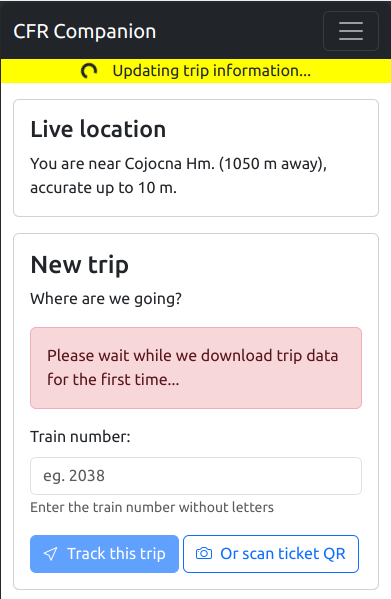
\includegraphics[width=.6\textwidth]{./figures/code/fe_update-banner.png}
    \caption{Frontend: the banner for when travel data is being updated.}
    \label{FigFeUpdateBanner}
\end{figure}

Various components need to know the state of the data update (whether it is checking for updates, what download decision has been taken, whether it is currently downloading or not, or whether it is the first time or not), so the state is provided to the entire application via a context. An usage example is visible in Figure \ref{FigFeUpdateBanner}, where the \textit{New trip} component displays a warning.

\subsection{Internationalization}
Internationalization was a fairly easy process, and it was done without using any third-party libraries. The way it works is by using a React context to provide the currently selected language, and then have the language provider \verb|LangProvider| provide a translation function.

The translation function takes in a translation key (eg. \verb|newTrip.trackBtn|), tries to find the translated string in the locale object (by parsing the object tree from the dot notation), and returns the translated string for use in JSX.

The translation function is reactively updated on changes to the selected language, such that it always returns values from the proper locale, and triggers UI updates across the component tree upon language selection.

In addition, the translation function takes any number of additional string parameters that get interpolated in the output string via numerical markers placed in the locale string (eg. \verb|$1|).

Another feature of the LangProvider is how it saves to the IDB store the currently selected language, and then, on application startup, it looks in IDB and loads up the last selected language. If it finds no selected language, it defaults to the user's navigator language, or English if that language is not recognized.

\begin{figure}[htbp]
    \centering
    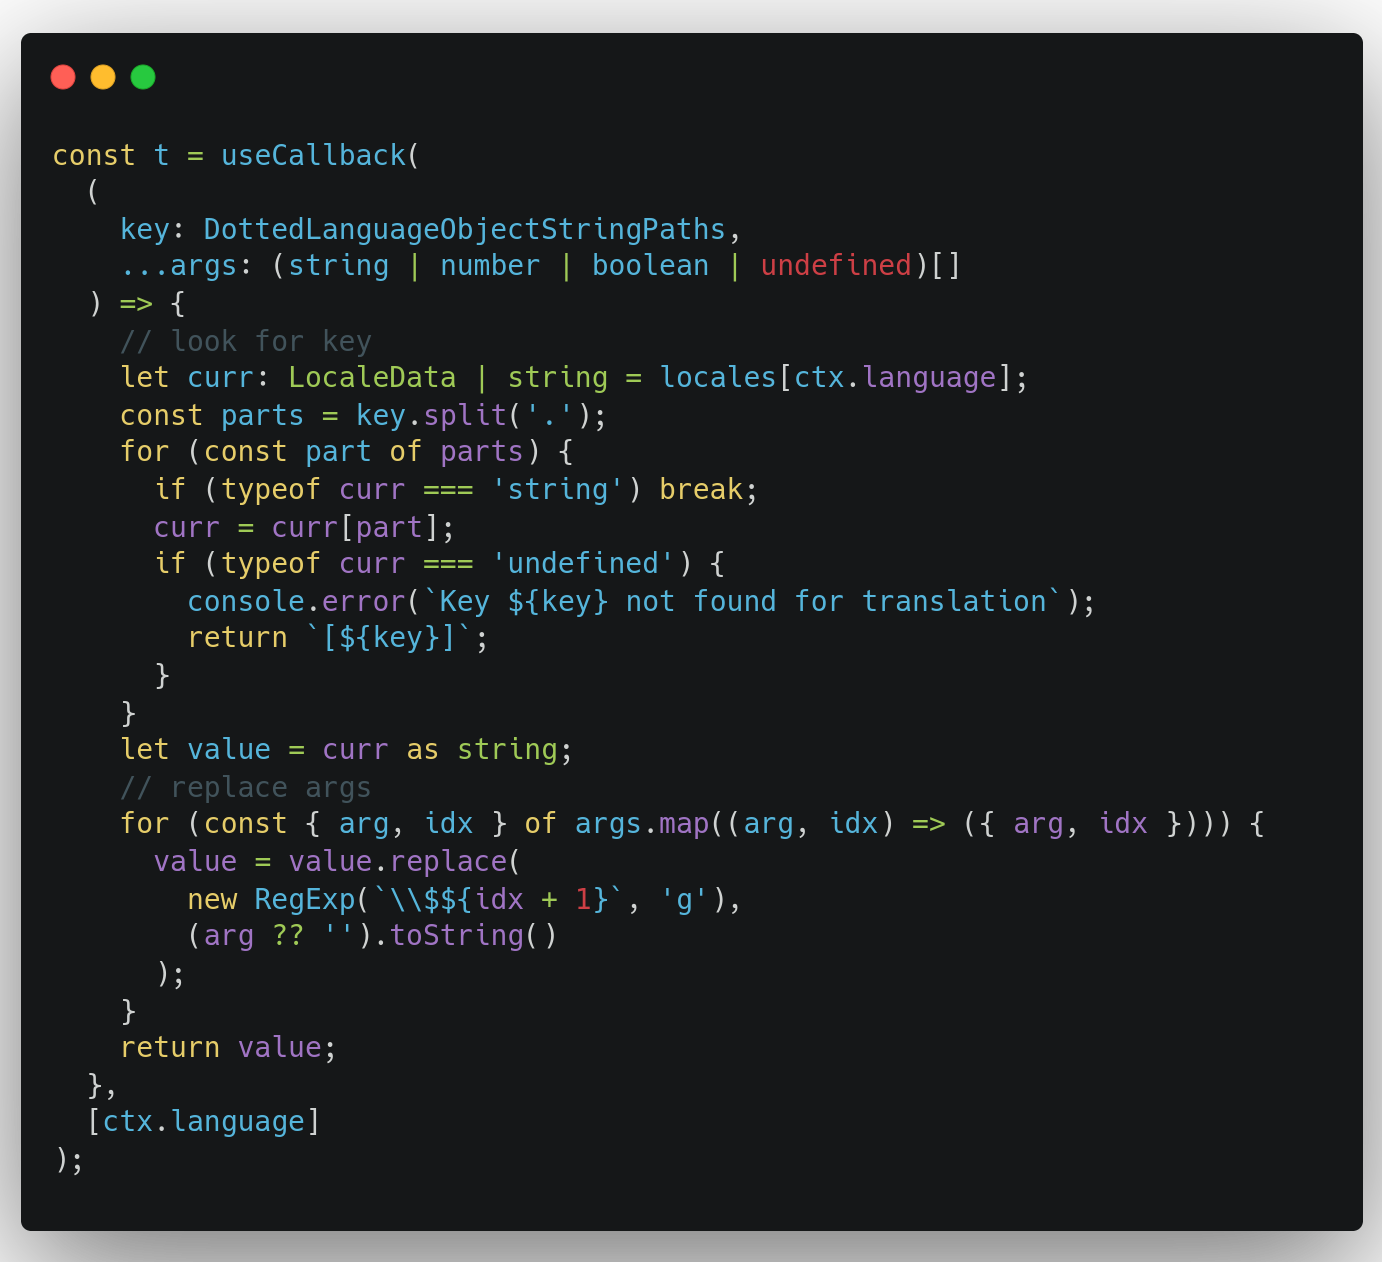
\includegraphics[width=.7\textwidth]{./figures/code/fe_translate-fn.png}
    \caption{Frontend: showcase of the translation function.}
    \label{FigFeTranslateFn}
\end{figure}

Figure \ref{FigFeTranslateFn} presents the translation function employed by the application. First\-ly, the function definition is wrapped in a React \verb|useCallback| hook, that will return the same function reference on subsequent renders (to help reactive code not react if nothing changed), but will return a different function reference when the \verb|ctx.language| value changes.

The function can be seen parsing the locale object of the currently selected locale (using the value of \verb|ctx.language|) and retrieving the proper locale string. If no such string is found, a default value of \verb|"[key]"| is provided.

Afterwards, the function will look in the arguments it has received and start replacing all occurrences of interpolation parameters with the proper values.

Once this process is done, the localized string is ready, and is returned.

An usage example of this translation function can be seen in the next subsection, in Figure \ref{FigFeLiveJsx}.

\subsection{Live location: nearest station}
On the home page, there exists a component whose role is to tell the user (using your live location) what station they are closest to, what distance separates them from it, and to what precision the app knows their location.

This is accomplished by running a query against the IDB GTFS store to retrieve all stations in Romania (totaling around 1700 stations) with their coordinates, calculating the distance to every one of those stations, then using the station with the lowest distance. This query is then repeated whenever a live location update occurs.

React's reactive way of writing application really shined in this context, since no special code had to be written to handle changes, because React simply took care of everything.

\begin{figure}[htbp]
    \centering
    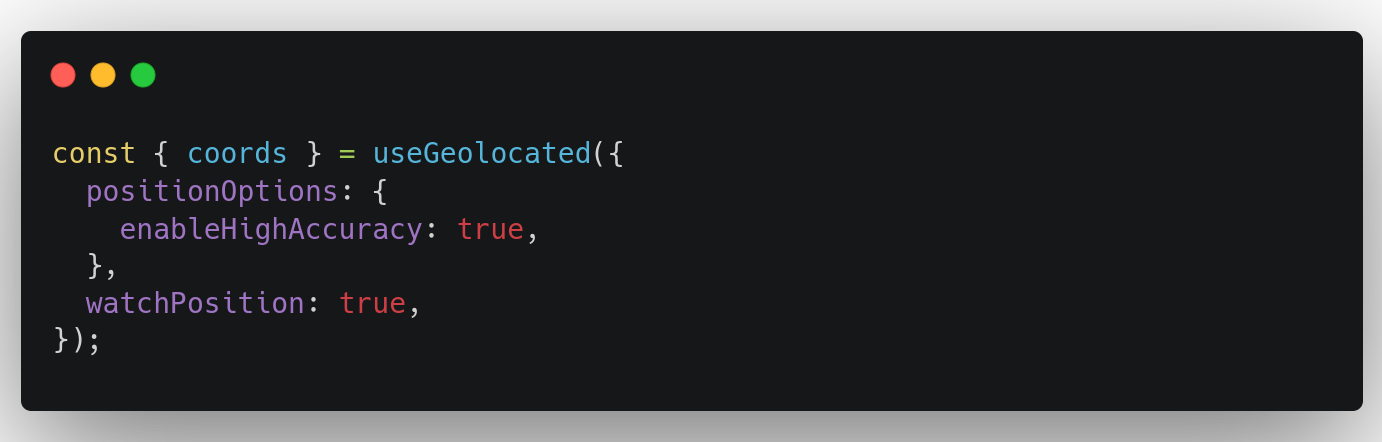
\includegraphics[width=.9\textwidth]{./figures/code/fe_live_coords.png}
    \caption{Frontend: usage of the useGeolocated hook to retrieve coordinates in real time.}
    \label{FigFeLiveCoords}
\end{figure}

Figure \ref{FigFeLiveCoords} shows how the \verb|react-geolocated|'s \verb|useGeolocated| hook was used to hook into the live location of the user. This hook will ask permission from the user to begin location tracking, then return the user's current location, while triggering re-renders every time this location updates.

\begin{figure}[htbp]
    \centering
    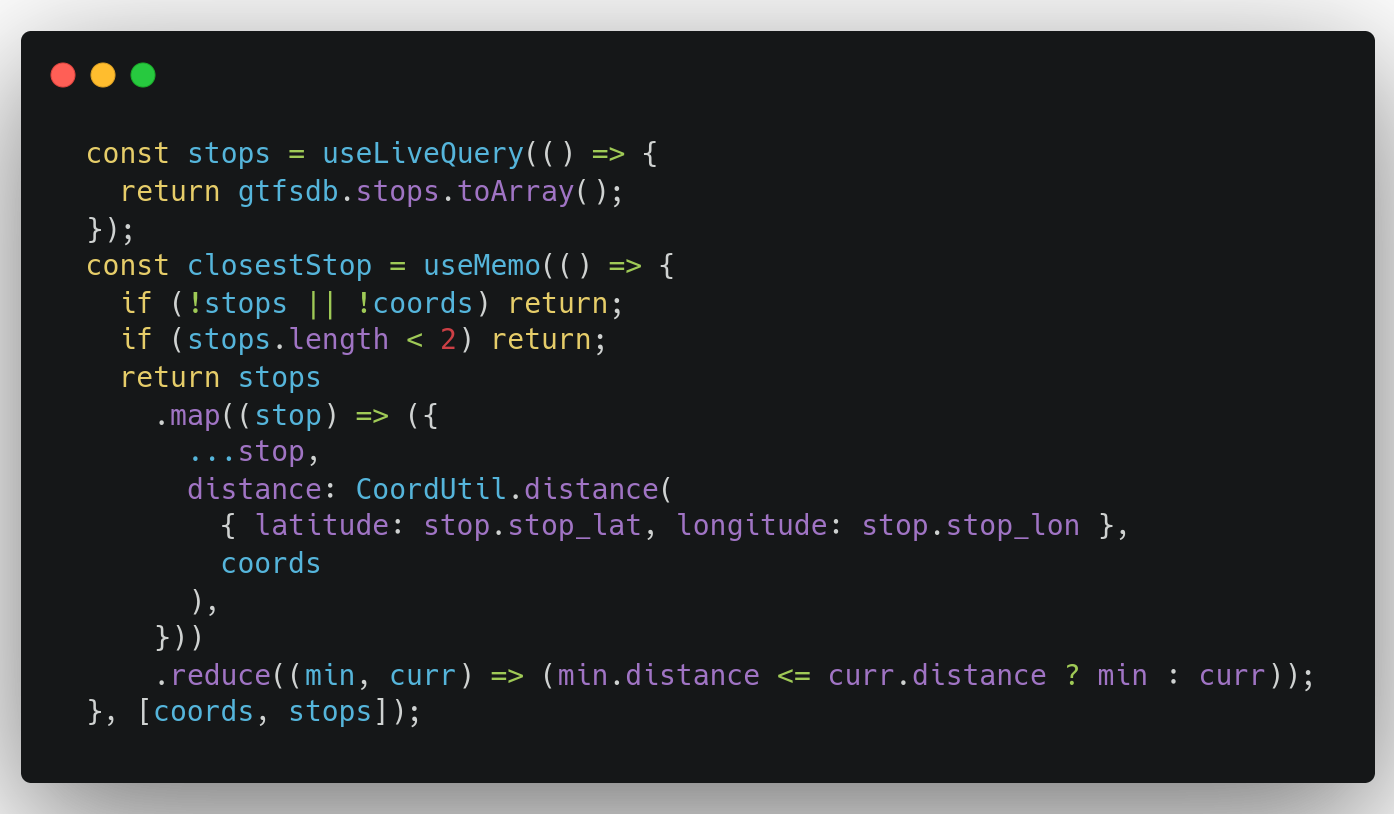
\includegraphics[width=.8\textwidth]{./figures/code/fe_live_queries.png}
    \caption{Frontend: usage of the useLiveQuery hook to retrieve always up-to-date data from IndexedDB.}
    \label{FigFeLiveQueries}
\end{figure}

Figure \ref{FigFeLiveQueries} shows how Dexie's \verb|useLiveQuery| hook is used to find all the stops and then React's \verb|useMemo| hook is used to recalculate the closest station only when either the list of stops or the user coordinates change. This figure exposes the ease with which array manipulation can be performed in JavaScript, using an easy, idiomatic, functional style of fluent function calls.

\begin{figure}[htbp]
    \centering
    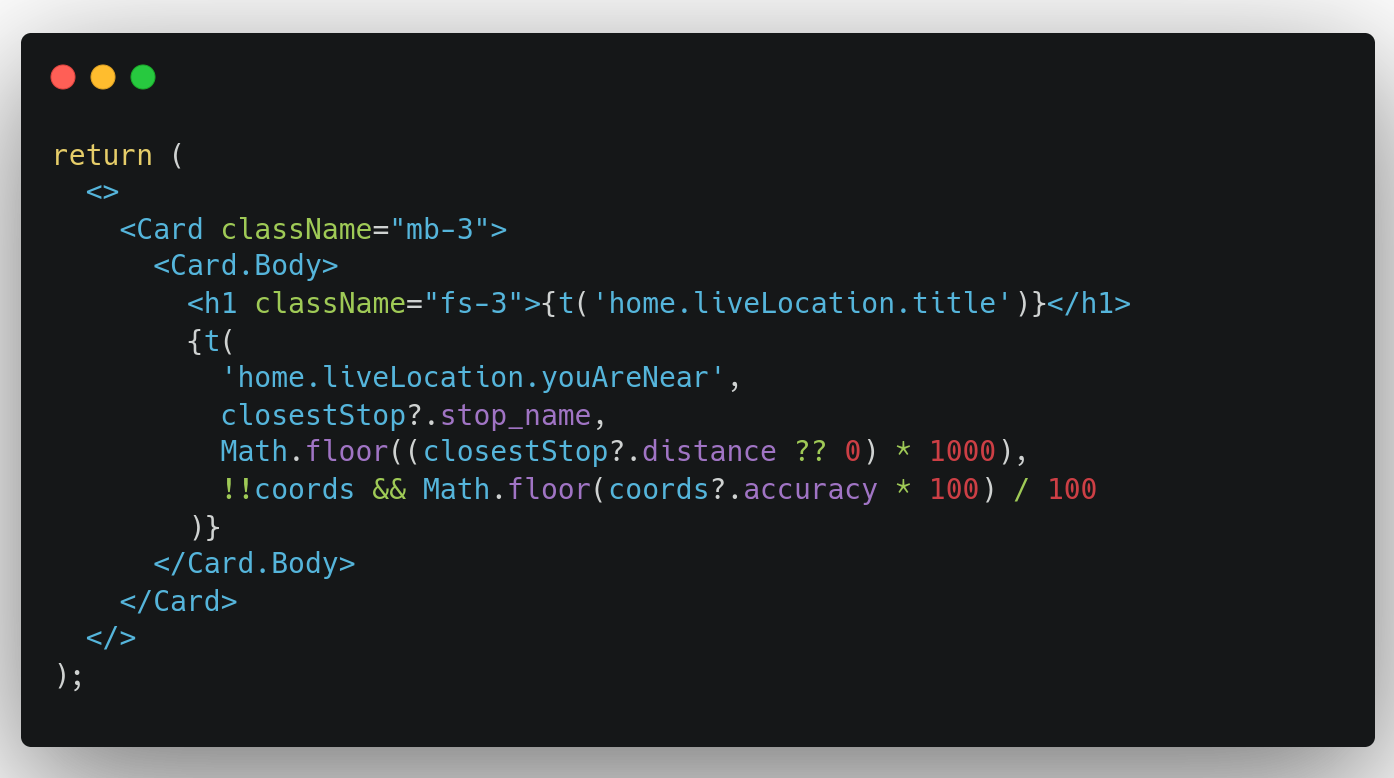
\includegraphics[width=.8\textwidth]{./figures/code/fe_live_jsx.png}
    \caption{Frontend: usage of the translation function in action, while showing, live, the nearest station to the user.}
    \label{FigFeLiveJsx}
\end{figure}

Figure \ref{FigFeLiveJsx} shows the return statement of the component, where the closest stop is displayed to the user by making extensive use of the translation function.

The reactive nature of the calculations really shine during GTFS travel data updates. While IndexedDB does not provide ways of notifying other code when data\-base updates happen, Dexie does keep track of database updates internally and therefore is able to hook into React's reactive system such that it automatically triggers function re-renders whenever relevant updates to the database happen. In this case, it can be seen how the component updates itself automatically when GTFS data is downloaded for the first time.

\subsection{Scanning ticket QR codes}
An important functionality of the application is the ability to scan QR codes located on physical tickets, and automatically figure out the user's current train, and destination.

While the meaning of the QR codes is not documented online, it was possible to reverse-engineer their meaning using a number of train tickets acquired over a period, and try to find out the meaning of each character in the decoded text.

\begin{figure}[htbp]
    \centering
    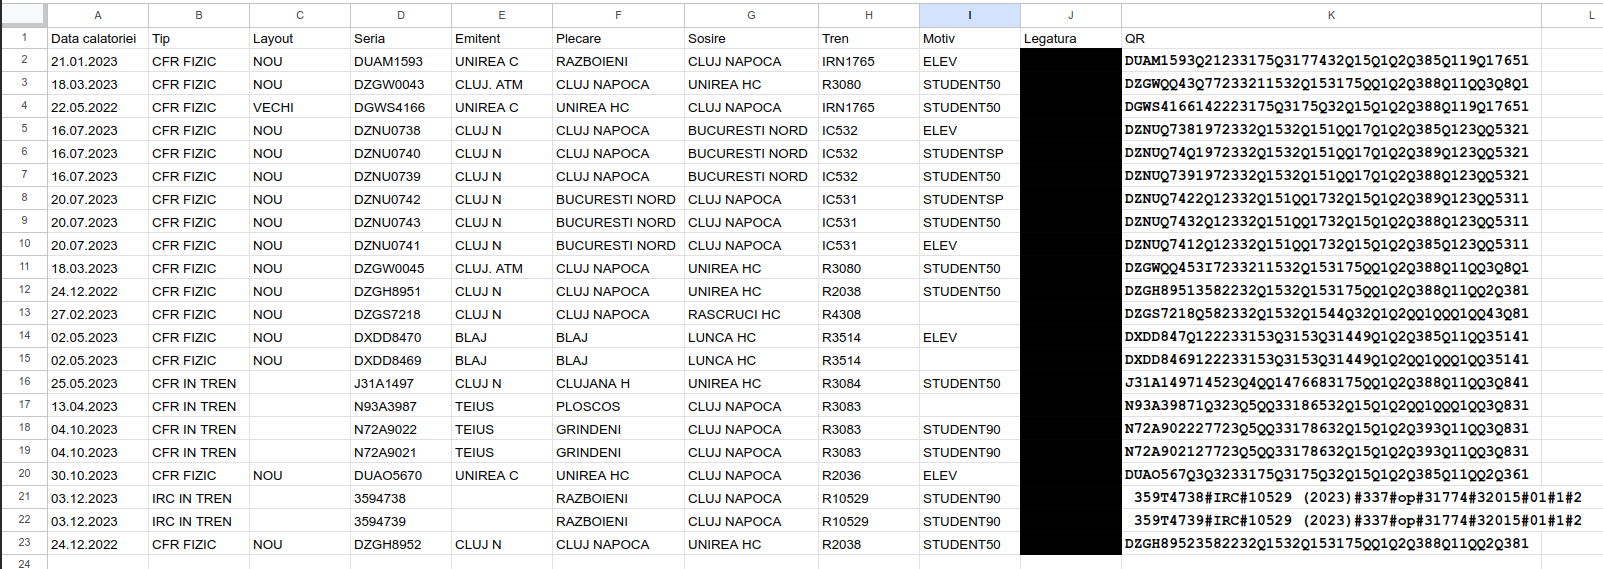
\includegraphics[width=1\textwidth]{./figures/ch4_cfr-tickets.png}
    \caption{Screenshot of the collection of train tickets I have collected for analysis, including two tickets for private operators. Personal information is censored.}
    \label{FigCfrTickets}
\end{figure}

Figure \ref{FigCfrTicketBreakdown} shows a breakdown of the different sections of a decoded ticket QR code. As a first step, we need to convert all \verb|Q| characters from the raw decoded data into zeroes, then we can process the different sections in the manner shown in the figure. It is easy, then, to determine what train the ticket refers to, the departure station, and the ticket's date.

\begin{figure}[htbp]
    \centering
    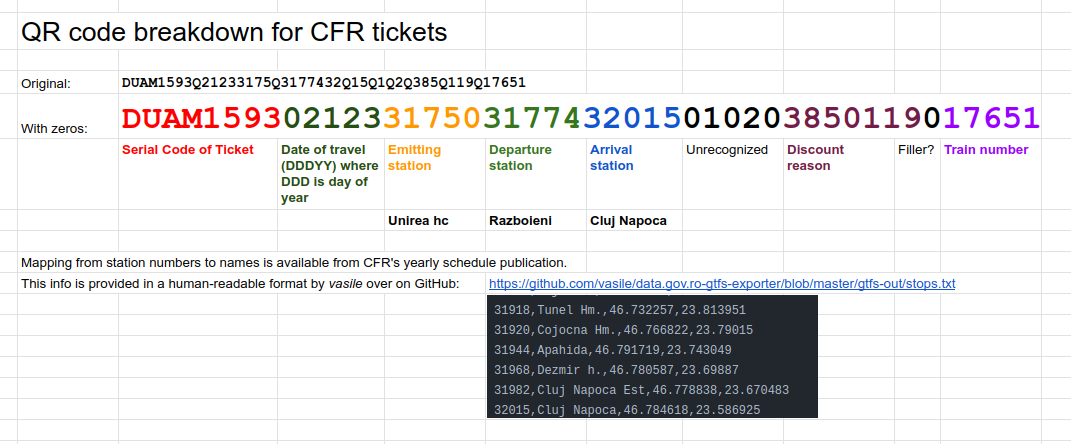
\includegraphics[width=1\textwidth]{./figures/ch4_cfr-ticket-breakdown.png}
    \caption{Breakdown of the QR code data of a CFR ticket.}
    \label{FigCfrTicketBreakdown}
\end{figure}

To integrate QR code scanning into our app, a library has been integrated with React, which performs QR code scanning and returns the raw string data. It is then easy to parse this data according to our rules, and redirect the user to the trip page.

\subsection{Live location: tracking a train}
Tracking a train is the entire point of the application. As a consequence, this feature is the most complex part of it. Let's begin by analyzing the two parts of the Track page: the live location illustration, and the timetable estimations.

\begin{figure}[htbp]
    \centering
    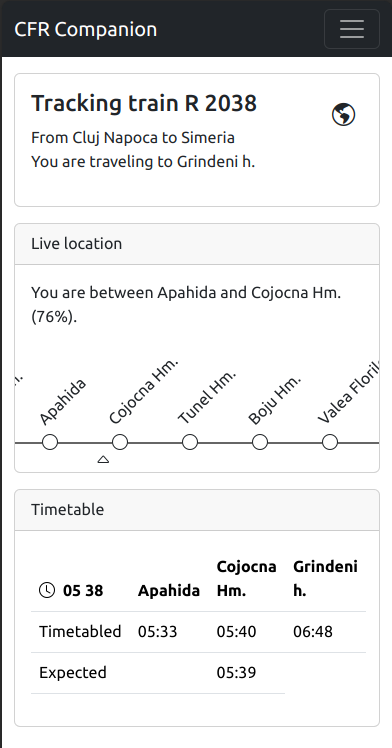
\includegraphics[width=.5\textwidth]{./figures/code/fe_track-all.png}
    \caption{Frontend: the tracking page, in its beautiful entirety.}
    \label{FigFeTrackAll}
\end{figure}

In Figure \ref{FigFeTrackAll}, at the top of the page, you can notice a section titled "Live location". This section displays the closest two stations to the user, and an illustration showing where the user is and what progress towards the next station they've made.

In the same figure, towards the bottom, a table provides arrival estimations for the next station, and the user's destination. The estimation is performed by taking the user's progress along the current leg, and relating it to when they should have departed from the last station, effectively creating an estimation for the train's delay in minutes, in real-time. An example of a two-minute delay is presented in Figure \ref{FigFeTrackWithDelay}.

\begin{figure}[htbp]
    \centering
    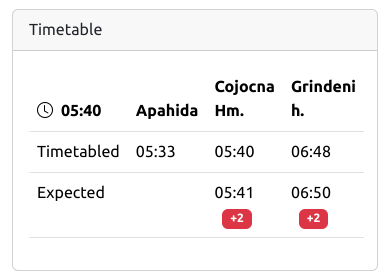
\includegraphics[width=.7\textwidth]{./figures/code/fe_track-with-delay.png}
    \caption{Frontend: how delays appear in the timetable estimations.}
    \label{FigFeTrackWithDelay}
\end{figure}

\subsection{PWA architecture}
Until now, we have described a normal React Single Page Application, that makes use of various browser features such as IndexFigFeTrackWithDelayedDB or live location. However, to turn this application into a PWA, we need to take some additional steps.

Firstly, we need to create an App Manifest. This is a plain JSON file that is used by the browser to determine important metadata about the application. It provides information such as the application name, description, preferred theme color, URL, or scope (path within the origin). This JSON file needs to be publicly accessible, and must be then referenced from the site's HTML using an appropriate \verb|link| tag.

Secondly, possibly the most important step of the process is to create a Service Worker. This service worker takes the form of a JS script that runs in a separate thread from the main page, and has the role of proxying all network requests originating from the main page. It has capability to manage browser caches and inject custom responses even when the network is not available. After creating the worker, it needs to be referenced in the main page's JS code via a Web API, which will enable the browser to register and bootstrap the service worker. This service worker will then persist its state across browser restarts, and across open tabs of the same site.

Thankfully, our bundler Vite provides handy tools to automate this process. Its \verb|vite-plugin-pwa| plugin offers a way of automatically look for the application's assets and create caching strategies for them.

\begin{figure}[htbp]
    \centering
    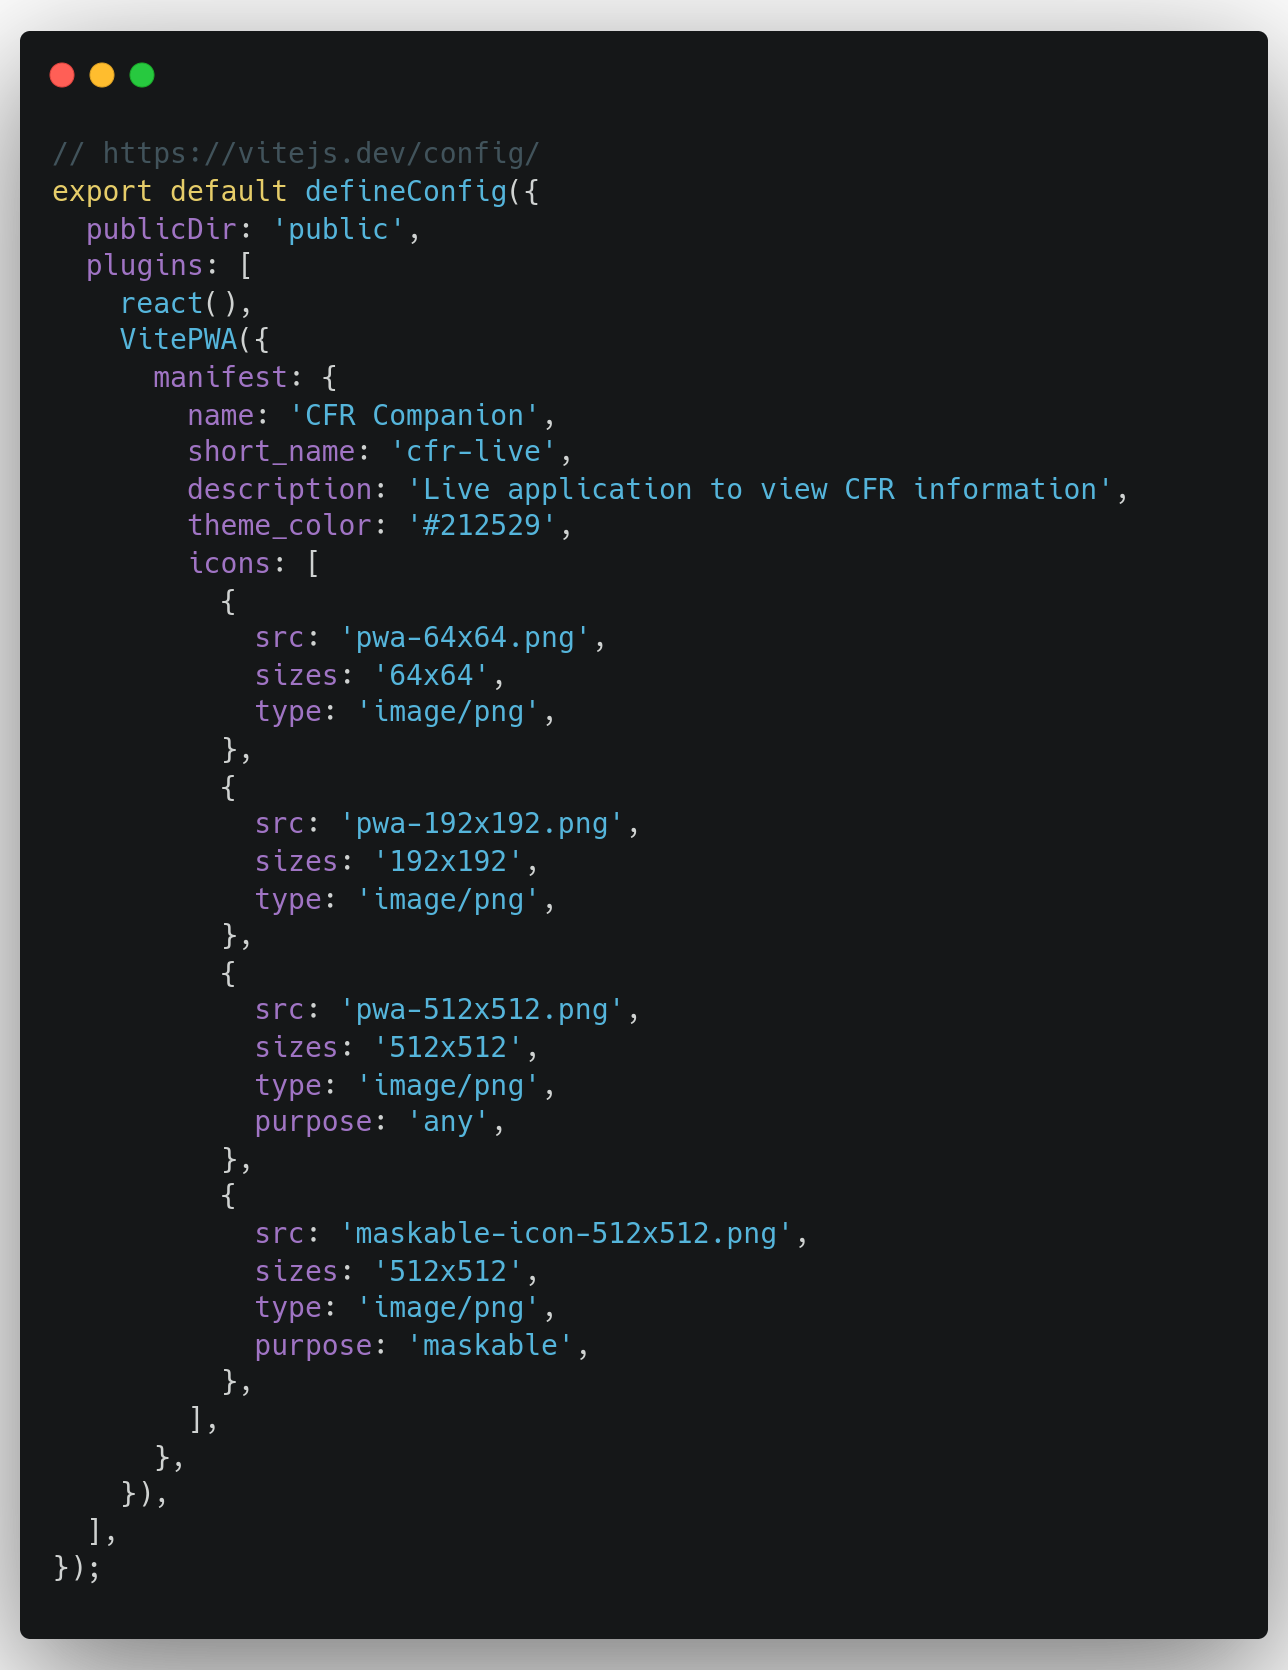
\includegraphics[width=.7\textwidth]{./figures/code/fe_vite-config.png}
    \caption{Frontend: how Vite is configured to produce a PWA-compliant build.}
    \label{FigFeViteConfig}
\end{figure}

Figure \ref{FigFeViteConfig} presents the configuration for the Vite PWA plugin. It takes as parameter only manifest data, which it cannot infer automatically (for obvious reasons). This is all it needs to produce a fully PWA-compliant build, since it can detect application assets (images) automatically.

\subsection{Offline functionality}
An important aspect of the PWA architecture lies in the offline functionality. While Internet connection is required on the first use of the application, it will automatically cache its resources and in the future will work offline out of the box. During this first use the GTFS data is also downloaded, such that train data will also be available offline.

However, certain functionalities require an internet connection to work, namely the authentication system.

To alleviate this issue, the application has code to handle the situation when API calls fail. While failure of API calls does not necessarily mean a lack of internet connection, it does mean that the online features of the application will not work regardless, so it is automatically treated as a "no internet" state.

When the application is not connected, a yellow banner is displayed, alerting the user, and offering the option of retrying. The "retry" button is important, since the app does not have a method of automatically realizing that connectivity is back.

At the same time, functionality that requires internet is hidden, such that the user can not log in anymore (or, if logged in, cannot log out). Additionally, a "no internet" icon is displayed next to the app name.

All this is done to alert the user to their lack of connectivity, but it should be understood that all features that do not explicitly require any API calls will still work, including, notably, usage of itinerary data.

\subsection{Frontend deployment}
The frontend deployment follows a similar constraint set to the ones presented in the counterpart section for the backend (Section \ref{sec:BeDeployment}). Therefore, the deployment flow is very similar.

The difference is notable only in the way the application is served. While the backend runs as a server, a Vite/React build only produces a set of static files, that require a separate server to be served to clients.

To this end, the \textit{nginx} setup on my personal VM helps, and it is configured to statically serve the build artifacts from Vite.

No special configuration is required for the static server to make the application PWA compliant, since the PWA registration is handled in a manner that is transparent to the static server.

\section{Testing}
With a limited scope and feature set, the application is suitable to be manually tested against the requirements outlined in Section \ref{sec:Requirements}.

To be able to test location-related features, I have personally taken builds of the application in various train trips, and noted down any bugs I have encountered. This process definitely helped, and it identified a couple of bugs I couldn't have found otherwise:

\begin{figure}[htbp]
    \centering
    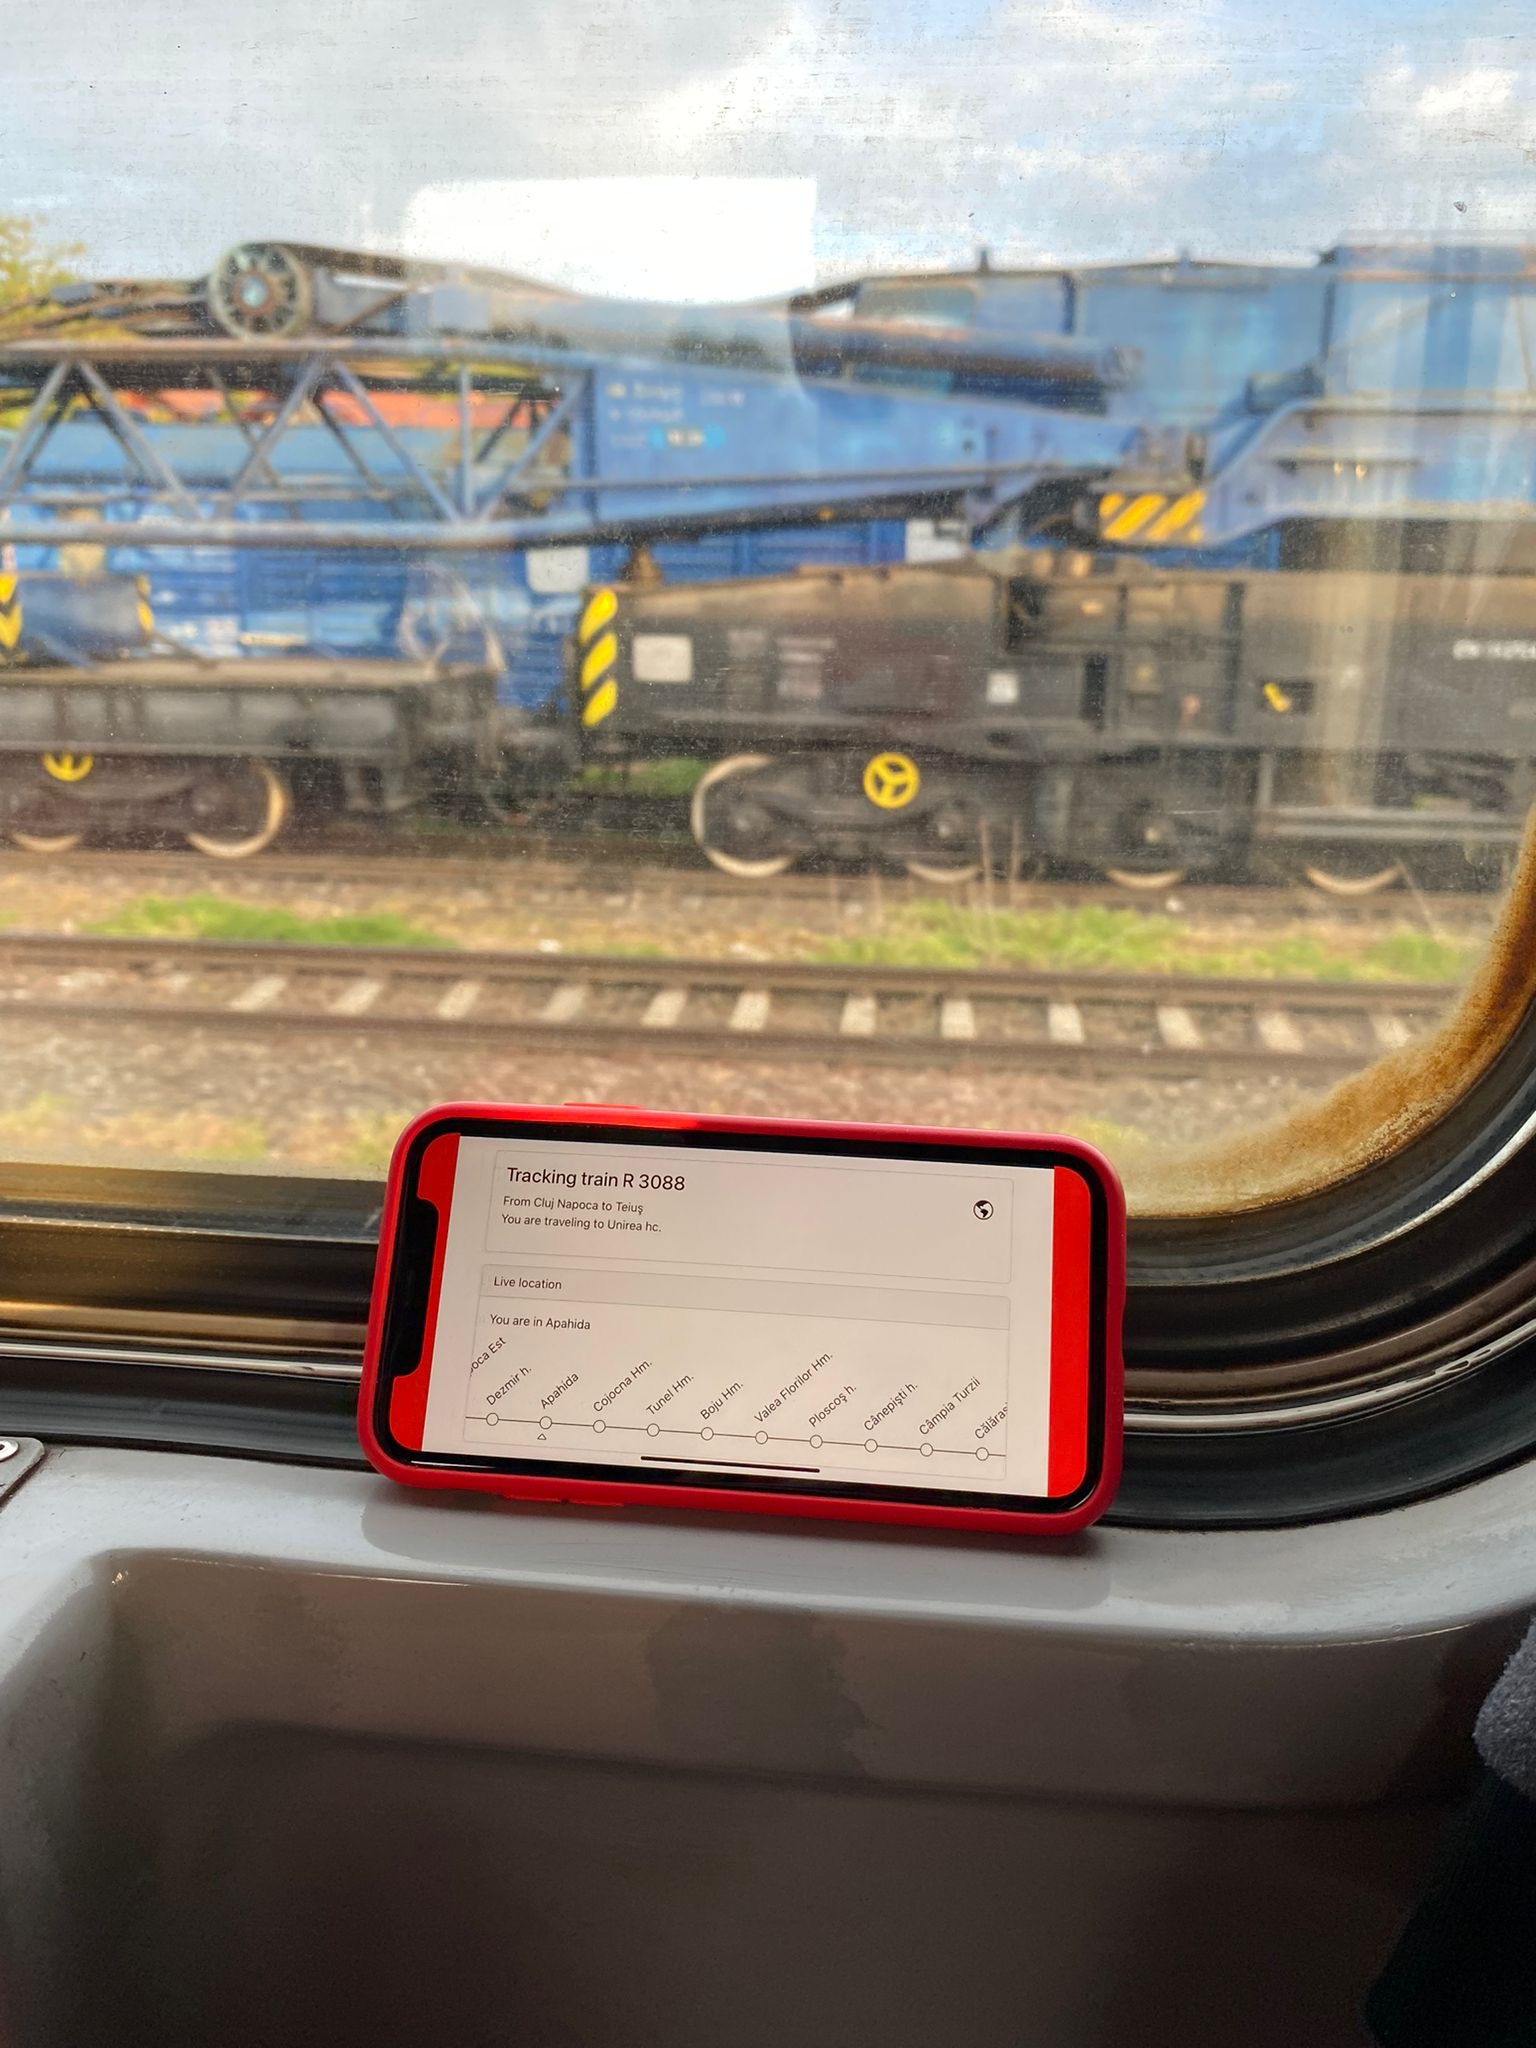
\includegraphics[width=.5\textwidth]{./figures/ch4_manual-testing.JPG}
    \caption{Manual testing of the application, during an actual train trip.}
    \label{FigManualTesting}
\end{figure}

\begin{itemize}
    \item There were instances where the closest two stations did not match up with the stations that you were between. This can happen whenever the station the user has last stopped in is further away than both of the next consecutive stations. To this end, the closest station calculation was modified to better reflect the user's current location relative to the stations.
    \item There were instances where the station coordinates did not match with the real-world location. This is a defect of the GTFS data set, and nothing short of case-by-case correction can be done about it.
    \item A need to automatically scroll the illustration arose from leaving the phone up for extended periods of time.
\end{itemize}